\chapter{ParticleFileWriter}
\label{chap:pfw}
\label{ch:pfw}
\index{ParticleFileWriter}
\index{pfwInput file}

\section{Purpose and generated products}
\label{sec:pfw-purpose}
\index{ParticleFileWriter!purpose}
\index{particle file}

The material point method solver tracks material state on Lagrangian particles and solves the equations of motion on an Eulerian background grid.  In GEOS-MPM, the background grid is constructed by the GEOS internal mesh generator, but the particles are created externally through a set of Python tools collectively referred to as the ParticleFileWriter, or \emph{PFW}.  As its name implies, the ParticleFileWriter creates the particle file: a plain-text description of the position, velocity, and geometry of each material point ``particle,'' along with auxiliary variables that define material type, contact group, surface state, particle type, and other optional properties.  This pre-processor exists as a separate Python toolset so that users can create custom configurations, geometries, and loading paths without editing or rebuilding the GEOS C++ source code.

PFW is therefore both a particle generator and a GEOS input generator.  Starting from a Python case definition, it writes
\begin{itemize}[leftmargin=*]
\item the particle file read by the \texttt{ParticleMeshGenerator};
\item the GEOS XML input containing the \texttt{InternalMesh}, \texttt{ParticleRegion}, constitutive blocks, solver block, finite-element space, events, diagnostics, and output blocks;
\item optional run scripts and scheduler settings; and
\item optional data or Python dependencies staged into the run directory.
\end{itemize}
The division of labor is intentional: GEOS owns the background grid and time integration, while PFW owns the initial particle state and the user-facing construction logic for nontrivial geometries.

\section{The \texttt{pfw\_input} file}
\label{sec:pfw-input}
\index{pfw input}
\index{pfw dictionary}
\index{Python input file}

A PFW case file is a Python file that is imported during case creation.  It can define any local Python variables, helper functions, classes, or objects needed to build the case.  Only data that must be passed to the PFW pre-processor, however, should be placed in the dictionary named \texttt{pfw}.  The dictionary is the contract between the case script and \texttt{particleFileWriter.py}.  Values outside the dictionary remain ordinary Python workspace variables used by the input script; values inside \texttt{pfw} are interpreted as PFW controls, particle-generation controls, or solver XML attributes.

The import-based design makes a \texttt{pfw\_input} file more flexible than a static keyword file.  Users commonly compute dimensions from parameters, loop over material definitions, read tabulated data, construct lists of geometry objects, or select between load cases before filling the final \texttt{pfw} dictionary.  PFW recognizes a set of predefined keys and also passes many unrecognized keys through as attributes on \texttt{SolidMechanics\_MPM}, after filtering known PFW-only metadata.  This pass-through behavior lets new solver controls be exercised before a dedicated PFW wrapper is added.

\begin{lstlisting}[language=Python,caption={Minimal shape of a PFW input file.}]
import numpy as np
import pfw_geometryObjects as geom
import pfw_materials as mat

# Local variables are allowed. They are not PFW inputs unless assigned to pfw.
refine = 2
cpp = 12
length = 1.0

pfw = {}
pfw["xmin"], pfw["xmax"] = -0.5*length, 0.5*length
pfw["ymin"], pfw["ymax"] = -0.5*length, 0.5*length
pfw["zmin"], pfw["zmax"] = -0.5*length, 0.5*length
pfw["xpar"], pfw["ypar"], pfw["zpar"] = refine, refine, refine
pfw["nI"], pfw["nJ"], pfw["nK"] = pfw["xpar"]*cpp, pfw["ypar"]*cpp, pfw["zpar"]*cpp
pfw["ppc"] = 2
pfw["endTime"] = 1.0e-5
pfw["outputType"] = "silo"       # or "vtk"
pfw["materials"] = [mat.elasticIsotropic("solid", rho=1000.0, E=1.0e6, nu=0.25)]
pfw["objects"] = [geom.box("block", mat=0, x0=[-0.4,-0.4,-0.4], x1=[0.4,0.4,0.4])]
\end{lstlisting}

The input file is imported as a module, so normal Python caveats apply.  Expensive work at module import time will be repeated whenever PFW imports the file.  For large geometry construction, users can put object generation in helper functions or use the \texttt{make\_objects} pattern supported by the current PFW script so that geometry construction can be restricted to the rank slice being generated.

\section{Input dependencies}
\label{sec:pfw-input-dependencies}
\index{pfw dependency}
\index{dependencies!PFW}

PFW supports two related dependency mechanisms: ordinary Python imports and explicit run-directory staging.  Ordinary imports are used for code that must be available while the \texttt{pfw\_input} file is executed; explicit staging is used for files that must be copied beside the generated case or made importable in the run directory.

\paragraph{Python and PFW helper imports.}
Most inputs import standard libraries, numerical packages, and PFW helper modules directly:
\begin{lstlisting}[language=Python,caption={Typical Python imports in a PFW input file.}]
import math
import numpy as np
import pfw_geometryObjects as geom
import pfw_materials as mat
from pfw_tracerPoints import disk, plane_grid, set_tracers
\end{lstlisting}
These imports are evaluated when \texttt{particleFileWriter.py} imports the input module.  The PFW run directory and the original input-file directory are inserted into \texttt{sys.path}, so local helper modules can also be imported if they are present or staged.

\paragraph{PFW dependency comments.}
Input files can request explicit file staging with comments of the form \texttt{\#[pfw\_dependency]}.  The current parser accepts paths relative to the original input directory, paths relative to the PFW directory, absolute paths, and optional destination paths inside the run directory:
\begin{lstlisting}[language=Python,caption={Examples of PFW dependency staging comments.}]
#[pfw_dependency] pfw_materials.py
#[pfw_dependency] input:tables/strength_table.csv
#[pfw_dependency] pfw:pfw_geometryObjects.py
#[pfw_dependency] /absolute/path/to/local_geometry.stl
#[pfw_dependency] input:tables/load_history.csv => tables/load_history.csv
\end{lstlisting}
A relative dependency first resolves relative to the original input-file directory and then falls back to the configured PFW directory for compatibility with older examples.  The \texttt{input:} prefix forces input-directory lookup, and the \texttt{pfw:} prefix forces lookup relative to the PFW installation directory.  A destination following \texttt{=>} is always relative to the run directory and cannot be absolute or contain \texttt{..}.  This is useful for material tables, STL files, tabulated load histories, Python helper modules, bitmap/voxel data, and post-processing scripts that should travel with a generated case.

\paragraph{Generated dependency list.}
After staging, PFW appends the staged paths to \texttt{pfw["dependencies"]}.  That list is workflow metadata and is filtered so that it does not become a solver XML attribute.  Rank zero stages files before the input module is imported on the other ranks, avoiding races on shared file systems.

\section{Background grid}
\label{sec:pfw-background-grid}
\index{background grid}
\index{InternalMesh}
\index{parallel mesh generation}
\index{plane strain!PFW}
\index{refinement!PFW}

PFW writes a GEOS \texttt{InternalMesh} for the background grid.  The main controls are the physical domain bounds \texttt{xmin/xmax}, \texttt{ymin/ymax}, \texttt{zmin/zmax}; the total cell counts \texttt{nI/nJ/nK}; periodic flags \texttt{periodic}; partition counts \texttt{xpar/ypar/zpar}; and particle-density controls \texttt{ppc}, \texttt{ppcx}, \texttt{ppcy}, and \texttt{ppcz}.  The generated mesh uses uniform Cartesian cells and the \texttt{C3D8} element type, even for plane-strain cases, because the MPM solver and particle mesh operate on the GEOS three-dimensional mesh data structures.

\subsection{Parallel grid-generation constraints}
\index{particles per partition}
\index{periodic boundaries!PFW grid}

The practical challenge in parallel PFW generation is to keep each MPI partition balanced while preserving a uniform grid and a simple particle-generation loop.  In typical production inputs, each partition is assigned the same number of cells in each active direction.  This means \texttt{nI}, \texttt{nJ}, and \texttt{nK} should be chosen consistently with \texttt{xpar}, \texttt{ypar}, and \texttt{zpar}.  Periodic and non-periodic directions differ slightly: non-periodic directions include one ghost cell on each side in the total \texttt{InternalMesh} count, whereas periodic directions do not add those two extra cells.  Consequently, PFW computes interior cell counts as
\begin{equation}
  n_x^{\mathrm{int}} =
  \begin{cases}
  N_x, & \text{periodic in }x,\\
  N_x-2, & \text{non-periodic in }x,
  \end{cases}
\end{equation}
and analogously for \(y\) and \(z\), except that plane strain always uses the reduced through-thickness treatment described below.  Thus, in a non-periodic direction, an input such as \texttt{nJ=3} means one physical/interior cell plus one buffer cell on each side, not three physical cells.  When an input parameter is intended to mean ``physical cells through the sample,'' set the PFW total cell count to that value plus two in each non-periodic direction:
\begin{lstlisting}[language=Python,caption={Converting physical cells to PFW total cells in a non-periodic direction.}]
physical_y_cells = 8
pfw["periodic"] = [False, False, False]
pfw["nJ"] = physical_y_cells + 2
\end{lstlisting}
The interior spacings are then
\begin{equation}
  \Delta x = \frac{x_{\max}-x_{\min}}{n_x^{\mathrm{int}}}, \qquad
  \Delta y = \frac{y_{\max}-y_{\min}}{n_y^{\mathrm{int}}}, \qquad
  \Delta z = \frac{z_{\max}-z_{\min}}{n_z^{\mathrm{int}}}.
\end{equation}

The appropriate number of particles per partition is hardware and model dependent.  A common CPU target is below roughly \(4\times 10^4\) particles per MPI partition for interactive development and moderate material complexity.  On GPU-enabled workflows, substantially larger partitions can be practical; values approaching \(10^6\) particles per partition may be usable for simple kernels and sufficiently large devices.  These are operational guidelines rather than solver limits: constitutive cost, contact fields, neighbor lists, output variables, and available memory can change the useful range by orders of magnitude.

\subsection{Common \texttt{cpp}--\texttt{refine}--\texttt{ppc} pattern}
\index{cells per partition}
\index{cpp}
\index{ppc}

Most suite and example inputs use a small set of derived variables rather than entering every mesh count directly.  The pattern is
\begin{align}
  \texttt{cpp} &= \text{cells per partition in a coordinate direction},\\
  \texttt{refine} &= \text{integer or real resolution multiplier},\\
  \texttt{xpar} &= \max(N_x^{\mathrm{pbc}},\, \mathrm{round}(\texttt{refine}\,\texttt{xpar0})),\\
  \texttt{nI} &= \texttt{xpar}\,\texttt{cpp},
\end{align}
with analogous definitions in \(y\) and \(z\).  Here \(N_x^{\mathrm{pbc}}\) is usually 3 in a periodic direction and 1 otherwise, so that periodic directions have enough partitions for periodic neighbor communication and representative partitioning.  The particle density is then set with \texttt{ppc} or direction-specific values.  With \texttt{ppc=2}, a full three-dimensional cell initially contains \(2^3=8\) candidate particle points before geometry filtering, while a plane-strain cell contains one through-thickness layer and \(2^2=4\) in-plane candidate points.

\begin{figure}[htbp]
  \centering
  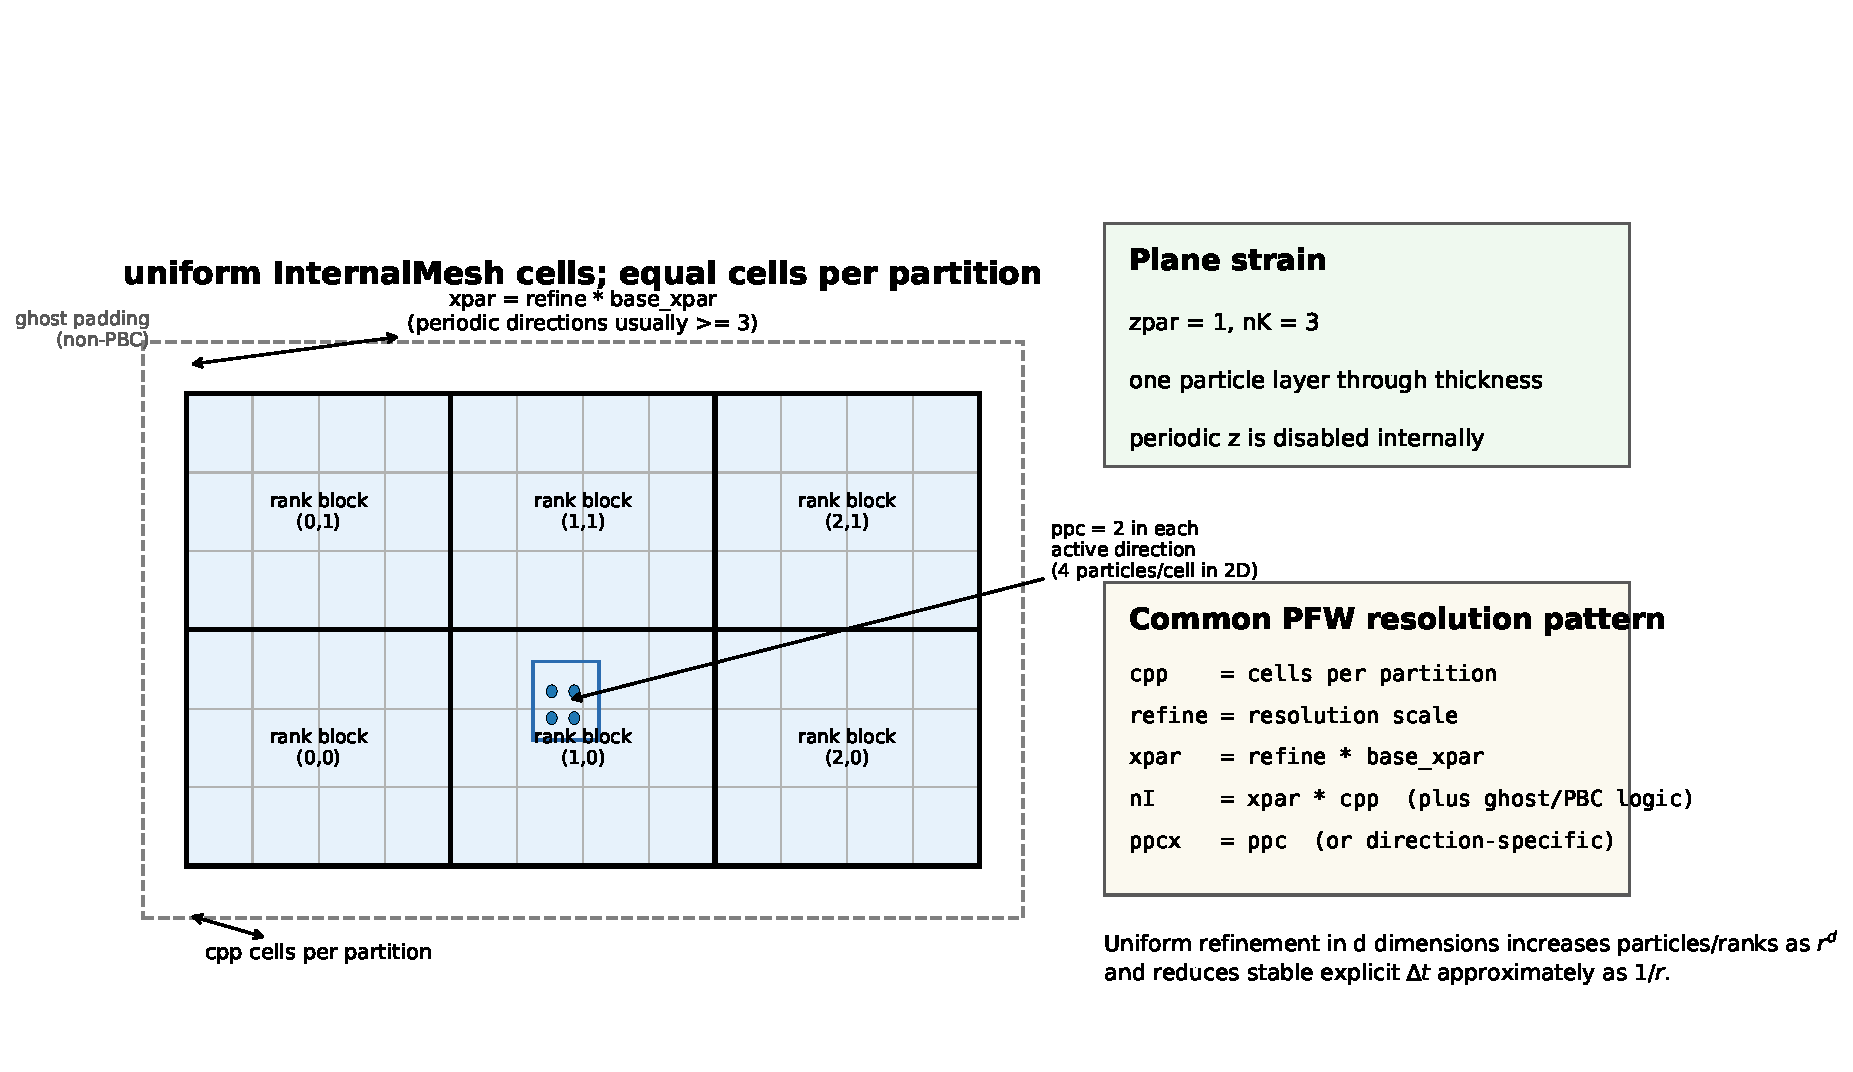
\includegraphics[width=0.92\linewidth]{figures/pfw_grid_partition_schematic.pdf}
  \caption{Typical PFW resolution pattern.  Users select a cells-per-partition count \texttt{cpp}, scale the number of partitions with \texttt{refine}, and choose particles per cell with \texttt{ppc}.  The resulting \texttt{InternalMesh} cells are uniform; non-periodic directions include ghost-cell corrections, while periodic directions generally require at least three partitions in production examples.}
  \label{fig:pfw-grid-partition-schematic}
\end{figure}

A representative input fragment is
\begin{lstlisting}[language=Python,caption={Resolution variables used to populate PFW mesh controls.}]
refine = 3
cpp = 12
base = [1, 1, 1]
pbc_min = [3 if p else 1 for p in pfw["periodic"]]

pfw["xpar"] = max(pbc_min[0], int(round(refine*base[0])))
pfw["ypar"] = max(pbc_min[1], int(round(refine*base[1])))
pfw["zpar"] = max(pbc_min[2], int(round(refine*base[2])))
pfw["nI"] = pfw["xpar"] * cpp
pfw["nJ"] = pfw["ypar"] * cpp
pfw["nK"] = pfw["zpar"] * cpp
pfw["ppc"] = 2
pfw["mCores"] = pfw["xpar"] * pfw["ypar"] * pfw["zpar"]
\end{lstlisting}

\subsection{Plane-strain meshes}
\index{plane strain!mesh}

Plane-strain cases are represented with a three-dimensional GEOS mesh but a reduced particle layer.  The current PFW checks
\begin{equation}
  \texttt{planeStrain}=1 \quad \Rightarrow \quad \texttt{zpar}=1, \qquad \texttt{nK}=3.
\end{equation}
PFW then treats the through-thickness direction as one active interior cell plus ghost padding, creates a single layer of particles through thickness, sets through-thickness particle velocities to zero, and passes \texttt{planeStrain} to the solver.  In-plane controls \texttt{ppcx} and \texttt{ppcy} still set the in-plane particle density; \texttt{ppcz} does not create multiple through-thickness layers in a plane-strain run.  The generated GEOS XML also disables periodicity in the suppressed \(z\) direction when \texttt{planeStrain}=1.

This representation keeps the same particle-file and mesh infrastructure as three-dimensional calculations while reducing the particle count and enforcing the intended kinematics.  Users should still choose a physical \(z\)-extent consistent with the constitutive model and any diagnostic interpretation of force, stress, or reaction quantities.

\subsection{Refinement and cost scaling}
\index{time step!refinement}
\index{CFL condition}
\index{cost scaling}

For explicit MPM, the stable time step scales with the cell size through the CFL condition.  If a fixed physical domain is refined by a factor \(r\) in each active direction, then \(\Delta x\sim r^{-1}\) and the number of steps required to reach a fixed physical time grows approximately as \(r\).  With fixed \texttt{ppc}, the particle count grows as \(r^d\), where \(d=2\) for plane-strain or other effectively two-dimensional calculations and \(d=3\) for full three-dimensional calculations.  The total explicit work to reach a fixed time therefore scales roughly as
\begin{equation}
  W(r) \propto r^{d+1},
\end{equation}
ignoring changes in contact, neighbor-list, constitutive, and communication overheads.  Thus a two-dimensional refinement sequence typically grows like \(r^3\) in total core work, and a three-dimensional sequence like \(r^4\).  If \texttt{cpp} is held fixed while \texttt{refine} increases the number of partitions, the per-rank particle count can remain approximately constant, but the number of time steps still grows as \(r\) and the total number of ranks grows as \(r^d\).  This is why PFW examples tend to expose \texttt{refine}, \texttt{cpp}, and \texttt{ppc} explicitly: the variables make accuracy, memory, and run-time tradeoffs visible in the input file.
\section{Geometry objects}
\label{sec:pfw-geometry-objects}
\index{Geometry objects}
\index{ParticleFileWriter!geometry objects}

PFW geometry objects are the particle-creation layer between a user-defined model and the plain-text particle file.  During particle generation, PFW loops over the candidate particle centers implied by the background grid and particle-density controls.  Each candidate point is tested against an ordered list of geometry objects.  The first object that accepts the point supplies the particle type, material index, contact group, initial velocity, and any optional fields requested in \texttt{particleFileFields}.  Objects can therefore create solid regions, leave voids, tag surface particles, assign different materials or contact groups, paint damage or porosity, prescribe material directions, and provide exact surface normals or surface positions for contact and cohesive-zone calculations.

\subsection{Creating objects and assembling the object list}
\index{objects@\texttt{objects}}
\index{make\_objects@\texttt{make\_objects}}
\index{geometry objects!creation}

The most direct workflow is to construct objects in the input file and assign the ordered list to \texttt{pfw["objects"]}.  The object order matters.  PFW tests objects sequentially and stops at the first match, so later objects do not overwrite particles created by earlier objects unless the earlier object rejects the particle point.  This priority rule is useful for inserting inclusions, defects, voids, or wrappers with controlled precedence.

\begin{lstlisting}[language=Python,caption={Assembling an explicit PFW object list.}]
import pfw_geometryObjects as geom

matrix = geom.box("matrix", x0=[-1.0,-1.0,-1.0], x1=[1.0,1.0,1.0], mat=0, group=0)
inclusion = geom.sphere("inclusion", x0=[0.0,0.0,0.0], r=0.25, mat=1, group=1)
void = geom.sphere("void", x0=[0.4,0.0,0.0], r=0.10, mat=-1, group=0)

# First accepted object wins.  Put small, high-priority features first.
pfw["objects"] = [void, inclusion, matrix]
\end{lstlisting}

When geometry construction is expensive or rank-dependent, the input module can instead define a function named \texttt{make\_objects}.  The current PFW script uses this function only when \texttt{pfw["objects"]} is absent.  A zero-argument \texttt{make\_objects()} function is the legacy form and constructs the full list on every PFW rank.  A two-argument form, \texttt{make\_objects(rankxmin, rankxmax)}, receives the approximate $x$-extent assigned to the current particle-generation rank and can construct only objects whose bounding boxes overlap that slice.  Some older notes and user inputs may refer to this pattern as a \texttt{makeObjects} option; the active Python hook in the reviewed code is \texttt{make\_objects}.

\begin{lstlisting}[language=Python,caption={Rank-sliced object construction with \texttt{make\_objects}.}]
def make_objects(rankxmin, rankxmax):
    objs = []
    for center, radius, mat, group in particle_database:
        if center[0] + radius < rankxmin:
            continue
        if center[0] - radius > rankxmax:
            continue
        objs.append(geom.sphere("grain", x0=center, r=radius, mat=mat, group=group))
    return objs
\end{lstlisting}

The rank-sliced form is particularly useful for granular beds, voxel-derived objects, Voronoi constructions, and other cases in which constructing all objects on every rank would dominate preprocessing time or memory.  It does not change the meaning of the final particle file; it only reduces the number of candidate objects that a rank constructs and tests.

\subsection{Object sorting in parallel PFW runs}
\index{sortObjects@\texttt{sortObjects}}
\index{geometry objects!sorting}
\index{parallel PFW!object sorting}

The \texttt{sortObjects} control is a second acceleration mechanism.  If \texttt{sortObjects=True}, PFW filters the object list at each candidate $x$-slice by evaluating
\begin{equation}
  x_{\min}^{(a)} \le x \le x_{\max}^{(a)},
\end{equation}
where \(x\) is the candidate particle center and \(x_{\min}^{(a)}\), \(x_{\max}^{(a)}\) are returned by object \(a\)'s \texttt{xMin()} and \texttt{xMax()} methods.  Only the filtered slice list is then searched for that $x$ coordinate.  The original order of the retained objects is preserved, so first-match priority is unchanged.

This option is intended for many-object geometries with compact bounding boxes, such as packed granular beds or collections of inclusions.  It is not enabled by default because some objects are unbounded, use infinite default bounds, or have only approximate \texttt{xMin}/\texttt{xMax} implementations.  Such objects remain correct when \texttt{sortObjects=False}; they simply do not benefit from $x$-slice filtering.  The two acceleration mechanisms are complementary: \texttt{make\_objects(rankxmin, rankxmax)} reduces object construction, while \texttt{sortObjects} reduces per-point object testing after the list has been constructed.

\subsection{Geometry-object interface and particle fields}
\index{geometry objects!interface}
\index{surface flags!PFW}
\index{getMat@\texttt{getMat}}
\index{getGroup@\texttt{getGroup}}
\index{isInterior@\texttt{isInterior}}

All PFW geometry objects are expected to provide at least an inside/outside query and enough metadata to assign particle fields.  The base \texttt{Geometry} constructor stores common attributes including \texttt{name}, \texttt{vel}, \texttt{mat}, \texttt{group}, \texttt{particleType}, \texttt{damage}, \texttt{porosity}, \texttt{temperature}, and \texttt{surfaceTraction}.  Objects can supply these as constants, callables, or explicit getter methods.

The central query is
\begin{equation}
  f_a(\mathbf{x}_p,h_s)=\texttt{object.isInterior(pt, skinDepth)},
\end{equation}
where \(\mathbf{x}_p\) is the candidate particle center and \(h_s\) is the surface-search depth computed from the cell and particle spacing.  A negative return value rejects the particle point.  A nonnegative return value accepts it and is interpreted as the particle's surface flag when the \texttt{SurfaceFlag} field is enabled.  The most common values are \texttt{0} for an interior particle, \texttt{1} for a fully damaged particle, \texttt{2} for a ordinary surface particle, \texttt{3} for a cohesive-zone surface particle, and \texttt{4} for a damaged cohesive particle.  Older comments and user discussions sometimes refer to an \texttt{isSurface} method; in the current particle-generation path the surface/interior decision is carried by the integer returned from \texttt{isInterior}.

After a candidate point is accepted, PFW queries optional object methods in the order required by the particle file.  Important methods and fallback attributes are summarized in Table~\ref{tab:pfw-geometry-interface}.  If a method is absent, PFW falls back to an attribute of the same concept, and if that attribute is callable it is evaluated at the particle point.  This pattern allows simple constant-valued objects and spatially varying user-defined objects to share the same interface.

\begin{table}[htbp]
\centering
\caption{Common PFW geometry-object attributes and methods.}
\label{tab:pfw-geometry-interface}
\small
\begin{tabularx}{\linewidth}{@{}p{0.31\linewidth}X@{}}
\toprule
\textbf{Attribute or method} & \textbf{Role in particle generation}\\
\midrule
\texttt{isInterior(pt, skinDepth)} & Accepts or rejects a candidate particle center.  Nonnegative return values become surface flags when the surface-flag particle field is written.\\
\texttt{xMin()}, \texttt{xMax()} & Bounding interval used by \texttt{sortObjects}; finite bounds improve sorting efficiency.\\
\texttt{getParticleType(pt)} or \texttt{particleType} & Selects single-point, B-spline, CPDI, CPTI, or CPDI2 particle type.\\
\texttt{getMat(pt)} or \texttt{mat} & Selects the material index written to the particle file.  A negative material index is used as a void/deletion convention and suppresses particle creation.\\
\texttt{getGroup(pt)} or \texttt{group} & Selects the contact group used by multi-field contact and related grouping options.\\
\texttt{getVelocity(pt)} or \texttt{vel} & Provides the initial particle velocity.  In plane strain, PFW forces the through-thickness component to zero.\\
\texttt{getDamage}, \texttt{getPorosity}, \texttt{getTemperature} & Assign optional initial state fields used by damage, porosity, and thermo-mechanical workflows.\\
\texttt{getSurfaceNormal(pt)} & Provides an explicit outward surface normal for contact, DFG, or cohesive-zone workflows when the particle is surface flagged.\\
\texttt{getSurfacePosition(pt)} & Provides the vector from the particle center to the exact or reconstructed surface point.\\
\texttt{getSurfaceTraction(pt)} & Provides an optional initial/external surface-traction vector for surface particles.\\
\texttt{getMatDir(pt)} & Provides a local material-direction triad for anisotropic materials, crystals, fibers, or layered strength fields.\\
\texttt{getStrengthScale(pt)} & Provides spatial strength scaling, often for Weibull or layered heterogeneity.\\
\texttt{getCZTag(pt)} & Provides cohesive-zone tags for surfaces that use cohesive constitutive models.\\
\texttt{getSubregions()} & Reports material/particle-type pairs so PFW can construct compatible \texttt{ParticleRegion} subregions.\\
\bottomrule
\end{tabularx}
\end{table}

The distinction between object geometry and object metadata is important.  The inside/outside test decides whether a particle exists; the getter methods decide how the accepted particle is interpreted by GEOS-MPM.  A geometry object can therefore be used as a solid inclusion, a void, a contact body, a material-orientation map, a cohesive surface generator, or a local state-field painter depending on which getters or wrappers are attached.

\subsection{Primitive analytic objects}
\index{geometry objects!analytic primitives}

\paragraph{\texttt{box}.}\index{geometry objects!box}Creates an axis-aligned rectangular solid from two opposite corners.  It is the most common object for blocks, platens, test coupons, and matrix domains.  Optional surface flags can enable or suppress selected faces for contact/cohesive workflows.

\paragraph{\texttt{box2}.}\index{geometry objects!box2}A box variant used primarily for contact testing.  It follows the same rectangular membership test as \texttt{box}, but uses mixed corner-normal behavior so that contact-normal handling can be exercised at edges and corners.

\paragraph{\texttt{notchedBar}.}\index{geometry objects!notchedBar}Creates a rectangular bar with an edge notch cut into the positive-$y$ face.  It is useful for fracture and localization examples that need a prescribed geometric flaw.  The source notes that notch surface normals are not fully defined, so exact-surface contact or cohesive workflows should verify this object before relying on those normals.

\paragraph{\texttt{sphere}.}\index{geometry objects!sphere}Creates a sphere from center and radius, returning surface flags and surface-normal/position data near the spherical boundary.  In two-dimensional or plane-strain examples it is commonly used as a disk-like cross-section when the through-thickness grid has one active layer.

\paragraph{\texttt{sphericalInclusion}.}\index{geometry objects!sphericalInclusion}Creates a spherical inclusion-like region but suppresses ordinary surface flagging.  This is useful when the inclusion should assign material or group data without creating a separate contact surface at the inclusion boundary.

\paragraph{\texttt{shell}.}\index{geometry objects!shell}Creates a spherical shell between inner and outer radii.  It marks particles lying between the two spherical surfaces and provides inward/outward surface data near the shell boundaries.

\paragraph{\texttt{ellipsoid}.}\index{geometry objects!ellipsoid}Creates a grid-aligned ellipsoid from a center and three semi-axis lengths.  It is useful for inclusions, pores, or idealized grains with anisotropic aspect ratios.

\paragraph{\texttt{cone}.}\index{geometry objects!cone}Creates a cone from two axis points and a base radius.  Surface normals distinguish the side wall and base, making the object useful for idealized tooling or conical inclusions.

\paragraph{\texttt{cylinder}.}\index{geometry objects!cylinder}Creates a solid or hollow cylinder from two axis points, an outer radius, and optionally an inner radius.  The object supports face/wall surface-flag controls, a slanted top plane through \texttt{n2}, and an axis-based material-direction triad.  Cylinders are used for disks, rods, pores, tools, and plane-strain circular samples.

\paragraph{\texttt{toroid}.}\index{geometry objects!toroid}Creates a toroidal annulus from a center, major radius, and minor radius.  It is useful for ring-like structures or curved voids.

\paragraph{\texttt{polygon}.}\index{geometry objects!polygon}Creates a two-dimensional polygon from ordered vertices.  PFW uses point-in-polygon and edge-distance operations to determine interior particles and surface flags.  The polygon is generally used for plane-strain domains or extruded cross-sections.

\paragraph{\texttt{porousPolygon}.}\index{geometry objects!porousPolygon}Extends \texttt{polygon} by inserting two-dimensional pores according to a porosity and pore-size specification.  It is used for plane-strain porous mesostructures where the outer boundary is polygonal.

\paragraph{\texttt{fill}.}\index{geometry objects!fill}Accepts all candidate particle points.  This is a convenience object for filling the full background domain or for constructing a lowest-priority background material beneath higher-priority objects.

\subsection{Tooling, sample, and test-fixture objects}
\index{geometry objects!tooling}

\paragraph{\texttt{indentor}.}\index{geometry objects!indentor}Creates a faceted, grid-aligned indentation tool from an apex/location, number of facets, and included angle.  Three facets approximate a Berkovich-style geometry and four facets approximate a Vickers-style geometry.

\paragraph{\texttt{spherical\_indenter}.}\index{geometry objects!spherical indenter}Creates an indenter with a spherical tip.  It is intended for indentation examples in which a curved contact surface is more appropriate than a faceted tip.

\paragraph{\texttt{flatpunch\_indenter}.}\index{geometry objects!flat punch indenter}Creates a flat-punch indenter with a specified radius and angle.  It is useful for verification of moving tools, boundary contact, and explicit contact surfaces.

\paragraph{\texttt{simple\_tensile\_gripper}.}\index{geometry objects!simple tensile gripper}Creates one side of a simple gripper claw for micromechanical tensile tests.  Dimensions define the inside width, grip height, gap, outer width, and thickness.

\paragraph{\texttt{tensile\_gripper}.}\index{geometry objects!tensile gripper}Creates a more detailed tensile gripper based on micromechanical test hardware dimensions.  It is used when the gripper itself is represented by particles rather than only by boundary conditions.

\paragraph{\texttt{pillar}.}\index{geometry objects!pillar}Creates a micropillar-style compression specimen with a cylindrical gauge length and a wider base connected by a smooth radial profile.  The object carries material-direction information and is intended for microcompression or strength-size-effect studies.  The source notes that its curved-surface normal approximation should be checked for exact-surface contact use.

\paragraph{\texttt{pillarBase}.}\index{geometry objects!pillarBase}Creates a supporting base geometry for pillar simulations.  It is typically paired with \texttt{pillar} to represent a substrate or pedestal beneath the gauge section.

\paragraph{\texttt{whiskers}.}\index{geometry objects!whiskers}Creates whisker- or fiber-like inclusions.  It is used for reinforced microstructure examples where slender embedded features need separate material directions or contact groups.

\subsection{Mesostructure and inclusion objects}
\index{geometry objects!mesostructures}

\paragraph{\texttt{crystal}.}\index{geometry objects!crystal}Generates a faceted crystal analogue from a center, axis, height, and minimum/maximum face offsets.  It is useful for synthetic crystal-like inclusions or grains with flat facets.

\paragraph{\texttt{foam}.}\index{geometry objects!foam}Creates a box with user-specified spherical pores.  The object removes particles inside the pore list and returns surface flags near the pore and outer-box boundaries.

\paragraph{\texttt{poissonDiskFoam}.}\index{geometry objects!poissonDiskFoam}Creates a grid-aligned foam block with pores sampled by a Poisson-disk-style algorithm.  It supports two-dimensional and three-dimensional modes, periodic sampling options, minimum-ligament constraints, and explicit surface-normal/position information.

\paragraph{\texttt{packedSphericalBed}.}\index{geometry objects!packedSphericalBed}Represents a packed bed of spherical grains inside a box.  The object stores grain centers, radii, material indices, contact groups, and particle types, and uses a cell-list search to answer point queries efficiently.  It can generate random sequential-addition-style packings or consume precomputed grain data provided through the input script.

\paragraph{\texttt{twoMaterialBox}.}\index{geometry objects!twoMaterialBox}Creates a box in which accepted particles randomly select between two material indices.  This is a simple stochastic mixture helper rather than a resolved microstructure generator.

\paragraph{\texttt{twoFieldBox}.}\index{geometry objects!twoFieldBox}Creates a box intended for two-contact-field or two-group testing.  It is a legacy/test helper for random or mixed contact group assignments; users should verify the current constructor before relying on it in production inputs.

\paragraph{\texttt{polygonInclusions}.}\index{geometry objects!polygonInclusions}Assigns particles to polygonal inclusions embedded in a surrounding fill group.  Polygons should be provided with counter-clockwise point ordering.  The object is useful for two-dimensional composite or mesoscale inclusion studies.

\subsection{Cohesive-zone and prill objects}
\index{geometry objects!cohesive zones}
\index{geometry objects!prills}

\paragraph{\texttt{czSphericalPrill}.}\index{geometry objects!czSphericalPrill}Creates a spherical prill containing Voronoi-like crystals separated by cohesive-zone surfaces.  It can assign contact groups, crystal material directions, surface positions, and cohesive tags needed by the cohesive-zone workflow.

\paragraph{\texttt{explicitBinderSphericalPrill}.}\index{geometry objects!explicitBinderSphericalPrill}Creates a two-dimensional spherical prill with explicit grain and binder regions.  It assigns grain and binder material indices separately and is used when binder ligaments should be represented by particles rather than only by cohesive interfaces.

\paragraph{\texttt{czCylindricalPrill}.}\index{geometry objects!czCylindricalPrill}Creates a cylindrical prill with Voronoi-like internal crystals and cohesive-zone surfaces.  It is appropriate for cylindrical or disk-like prill geometries where cohesive interfaces are inserted between neighboring grains.

\paragraph{\texttt{czPrill}.}\index{geometry objects!czPrill}Creates a box-shaped prill with internal Voronoi crystals, cohesive-zone tags, and configurable bonded/neat surface fractions.  It is a general prill mesostructure object for cohesive fracture and contact studies.

\subsection{Voxel, image, and surface-import objects}
\index{geometry objects!voxel imports}
\index{geometry objects!STL}
\index{geometry objects!image-based}

\paragraph{\texttt{stl}.}\index{geometry objects!stl}Imports a closed triangulated STL surface.  The object supports ASCII and binary STL files, translation, scaling, optional centering, normal flipping, ray-casting inside/outside tests, and nearest-triangle surface projection.  It is useful for CAD-derived or segmented geometries that are not easily represented by analytic primitives.

\paragraph{\texttt{VCCTL}.}\index{geometry objects!VCCTL}Creates particles from a VCCTL-style voxelized dataset.  Integer voxel phase values are mapped to material indices through a user-supplied map, allowing cementitious or other voxel-resolved microstructures to be converted into particles.

\paragraph{\texttt{CT}.}\index{geometry objects!CT}Creates particles from a three-dimensional computed-tomography voxel dataset.  It is similar to \texttt{VCCTL} but kept separate for compatibility and specialization of CT-generated arrays and phase maps.

\paragraph{\texttt{bitmap}.}\index{geometry objects!bitmap}Creates a two-dimensional particle geometry from an image or binary array.  Pixel or label values map to material indices, making this object useful for plane-strain image-based mesostructures.

\paragraph{\texttt{GrainStack}.}\index{geometry objects!GrainStack}Creates particles from a stacked voxel or labeled-array representation of grains.  It provides bounding-box and index-casting utilities for converting array coordinates into model-space particles.

\subsection{Periodic and architected-structure objects}
\index{geometry objects!architected structures}

\paragraph{\texttt{spinodal}.}\index{geometry objects!spinodal}Creates a spinodal-like porous or bicontinuous structure from a random field and target density controls.  It returns surface data by projecting to the implicit surface and is useful for synthetic porous materials.

\paragraph{\texttt{tpms}.}\index{geometry objects!tpms}Creates triply periodic minimal surface or related periodic architectures using a selected implicit surface type, target density, cell size, and offset.  It is used for gyroid-like, Schwarz-like, spinodal, or other periodic mesostructures.

\subsection{Boolean set operations}
\index{geometry objects!Boolean operations}
\index{union@\texttt{union}}
\index{intersection@\texttt{intersection}}
\index{difference@\texttt{difference}}

The Boolean objects combine two existing geometry objects while preserving the PFW query interface.  They are useful for creating holes, clipped inclusions, intersected tool shapes, and domains assembled from reusable primitives.

\paragraph{\texttt{union}.}Accepts a particle point if either sub-object accepts it.  Surface data are inherited from the sub-object that controls the accepted point according to the operation's priority rules.

\paragraph{\texttt{intersection}.}Accepts a particle point only if both sub-objects accept it.  This is useful for clipping one object by another, such as retaining only the portion of a cylinder inside a box.

\paragraph{\texttt{difference}.}Accepts particles that are inside object \texttt{A} and outside object \texttt{B}.  This is the standard tool for cutting voids, pores, holes, or notches from an otherwise solid object.  The current implementation includes surface-normal and surface-position logic to decide whether the nearest retained boundary belongs to \texttt{A} or to the removed object \texttt{B}.

\subsection{Geometry wrappers and field painters}
\index{geometry objects!wrappers}
\index{wrappers!geometry}

Wrappers take a sub-object and override or augment one part of its response.  They are the preferred way to add field data without reimplementing an inside/outside test.  All wrappers forward unmodified queries to the wrapped object unless they specifically override that field.

\paragraph{Basic field wrappers.}The wrappers \texttt{materialDirectionWrapper}, \texttt{surfaceFlagWrapper}, \texttt{czTagWrapper}, \texttt{surfaceNormalWrapper}, \texttt{surfacePositionWrapper}, \texttt{shrinkageFlagWrapper}, \texttt{strengthScaleWrapper}, \texttt{damageWrapper}, \texttt{porosityWrapper}, and \texttt{temperatureWrapper} assign a corresponding constant or callable value to particles accepted by the wrapped object.

\paragraph{Deletion and masking wrappers.}\texttt{functionalDeletionWrapper} calls a user-supplied deletion function and rejects points that should be removed.  \texttt{pointwisePorosityWrapper} randomly suppresses a fraction of points to represent unresolved porosity, but does not construct deterministic pore surfaces or surface flags.

\paragraph{Voronoi, Weibull, and material-direction wrappers.}\texttt{voronoiWrapperWithLayeredStrengthScale}, \texttt{layeredVoronoiWeibullWrapper}, \texttt{voronoiWeibullBoxWrapper}, \texttt{voronoiMatDirBoxWrapper}, \texttt{sizeEffectVoronoiWeibullBoxWrapper}, and \texttt{layeredStrengthScaleBoxWrapper} assign spatially varying material directions, strength scales, flaws, or layered Weibull fields.  These wrappers are used for heterogeneous strength distributions, grain-level anisotropy, and size-effect studies.

\paragraph{Box-local and crack-like wrappers.}\texttt{surfaceFlagBoxWrapper} and \texttt{damageBoxWrapper} override surface flag or damage only inside a specified box.  \texttt{pennyShapedCrackWrapper} paints a penny-shaped damaged region defined by two points and a radius, making it useful for seeded-crack or pre-damage studies.

\paragraph{Coordinate-transform wrapper.}\texttt{transform} maps query points through a user-supplied transform before delegating to the sub-object, and transforms returned normals or vectors as needed.  It allows an analytic or imported object to be translated, rotated, or otherwise mapped without creating a new object class.
\section{Materials, groups, and particle types}
\label{sec:pfw-materials}
\index{materials}
\index{groups}
\index{particle types}
\index{MaterialType@\texttt{MaterialType}}
\index{ContactGroup@\texttt{ContactGroup}}
\index{ParticleType@\texttt{ParticleType}}

This section describes how PFW assigns the particle-level integers and optional orientation data that connect a generated particle file to the solver-side material, contact, and interpolation algorithms.  Constitutive-model equations and integration details are described in Section~\ref{sec:constitutive}; particle interpolation and update schemes are described in Section~\ref{sec:particle-types-and-mapping}; and multi-field, DFG, and explicit-surface contact options are described in Section~\ref{sec:contact-options}.  The purpose of this PFW section is narrower: it documents how the input script and geometry objects choose the values that are written into the particle file.

PFW can generate particle files for several solver material-model families.  The current source-derived catalogue includes the models listed in Table~\ref{tab:pfw-material-model-list}.  Only the model names are listed here because the physics, parameters, and calibration guidance belong in the constitutive-model documentation and linked material-model reports.

\begin{table}[htbp]
\centering
\caption{Solver material-model families visible to PFW in the reviewed source tree.  See Section~\ref{sec:constitutive} and Appendix~\ref{app:geometry-materials} for the generated catalogue.}
\label{tab:pfw-material-model-list}
\small
\begin{tabularx}{\linewidth}{@{}p{0.30\linewidth}X@{}}
\toprule
\textbf{Family} & \textbf{Model names}\\
\midrule
Elastic and anisotropic elastic & \texttt{ElasticIsotropic}, \texttt{ElasticTransverseIsotropic}, \texttt{ElasticTransverseIsotropicPressureDependent}.\\
Plasticity and hyperelasticity & \texttt{VonMisesJ}, \texttt{PerfectlyPlastic}, \texttt{Hyperelastic}, \texttt{HyperelasticMMS}.\\
Damage, polymers, graphite, and geomaterials & \texttt{CeramicDamage}, \texttt{Chiumenti}, \texttt{StrainHardeningPolymer}, \texttt{Graphite}, \texttt{Geomechanics}.\\
Cohesive-zone materials & \texttt{BicrystalCohesiveZone}, \texttt{CoupledCohesiveZone}, \texttt{PolymerCohesiveZone}; see Section~\ref{sec:cohesive-zone-implementation}.\\
\bottomrule
\end{tabularx}
\end{table}

\subsection{Particle-level assignments made by geometry objects}
\label{subsec:pfw-material-group-type-assignment}
\index{geometry objects!material assignment}
\index{geometry objects!contact group assignment}
\index{geometry objects!particle type assignment}

Each accepted particle receives three core classification values:
\begin{align}
  m_p^{\mathrm{PFW}} &= \texttt{MaterialType},\\
  g_p^{\mathrm{PFW}} &= \texttt{ContactGroup},\\
  \tau_p^{\mathrm{PFW}} &= \texttt{ParticleType}.
\end{align}
The first two are ordinary particle-file columns when \texttt{MaterialType} and \texttt{ContactGroup} are present in \texttt{particleFileFields}; the particle type is used by PFW while building particle blocks and by the generated \texttt{ParticleMesh} XML entry.  In the reviewed PFW code, the standard particle-type integers are
\begin{center}
\begin{tabular}{@{}cl@{}}
\toprule
\textbf{Integer} & \textbf{Solver particle type}\\
\midrule
0 & \texttt{SinglePoint}\\
1 & \texttt{SinglePointBSpline}\\
2 & \texttt{CPDI} (current PFW default)\\
3 & \texttt{CPTI} placeholder\\
4 & \texttt{CPDI2} placeholder\\
\bottomrule
\end{tabular}
\end{center}

The \texttt{mat} value is a zero-based index into \texttt{pfw["materials"]}.  If \texttt{pfw["materials"] = ["matrix", "inclusion"]}, then \texttt{mat=0} assigns the particle to the \texttt{matrix} material and \texttt{mat=1} assigns it to \texttt{inclusion}.  PFW groups particles with the same material index into separate generated \texttt{ParticleRegion} entries whose \texttt{materialList} names come from \texttt{pfw["materials"]}.  The corresponding material XML snippets must be present in \texttt{pfw["materialPropertyString"]}; Section~\ref{subsec:pfw-material-library} gives examples using \texttt{pfw\_materials.py}.

The \texttt{group} value is the contact-group or material-field label used by the solver contact algorithms.  For prescribed multi-field contact, particles in different groups can map to different nodal velocity fields and interact through the contact update described in Section~\ref{sec:contact-options}.  For DFG contact, the prescribed group is the base field label and the damage-field-gradient split creates additional side fields internally.  The group label is therefore a kinematic/contact classification, not a constitutive material selection; it is common for two particles to share the same material index but have different contact groups, or to have different material indices but the same contact group when no material-field separation is intended.

The \texttt{particleType} value selects the mapping and domain representation described in Section~\ref{sec:particle-types-and-mapping}.  It can be used uniformly for an entire object, or varied by object to mix, for example, CPDI particles in deformable solids with single-point particles in simple fixtures.  Mixing particle types should be deliberate because the particle type controls stencil size, surface/domain geometry, and allowable future options.

\begin{lstlisting}[language=Python,caption={Constant material, group, and particle-type assignments on geometry objects.}]
import pfw_geometryObjects as geom

# Particle type integers: 0 SinglePoint, 1 SinglePointBSpline,
# 2 CPDI, 3 CPTI placeholder, 4 CPDI2 placeholder.
matrix = geom.box("matrix",
                  x0=[-1.0,-1.0,-1.0], x1=[1.0,1.0,1.0],
                  mat=0, group=0, particleType=2)

inclusion = geom.sphere("inclusion",
                        x0=[0.0,0.0,0.0], r=0.25,
                        mat=1, group=1, particleType=2)

pfw["objects"] = [inclusion, matrix]
pfw["materials"] = ["matrixElastic", "inclusionCeramic"]
\end{lstlisting}

PFW obtains these values by querying the accepted object.  If an object provides \texttt{getMat(pt)}, \texttt{getGroup(pt)}, or \texttt{getParticleType(pt)}, those methods are used.  Otherwise PFW falls back to the object attributes \texttt{mat}, \texttt{group}, and \texttt{particleType}; callables are evaluated at the particle point where supported by the current code path.  Objects that can emit multiple material/type combinations should also implement \texttt{getSubregions()} so PFW can build the complete \texttt{ParticleMesh} block list before the particle file is written.  The default implementation returns one pair, \texttt{[(mat, particleType)]}; multi-material objects such as packed beds, voxel imports, and stochastic mixtures override this to enumerate all possible \((\texttt{mat},\texttt{particleType})\) pairs.

\begin{lstlisting}[language=Python,caption={Spatially varying material and group assignment through object methods.}]
class LayeredBox(geom.box):
    def getMat(self, pt):
        return 0 if pt[1] < 0.0 else 1

    def getGroup(self, pt):
        return 10 if pt[0] < 0.0 else 11

    def getSubregions(self):
        # PFW needs all material/type pairs before particle generation.
        return [(0, self.particleType), (1, self.particleType)]

obj = LayeredBox("layered", x0=[-1,-1,-1], x1=[1,1,1], particleType=2)
pfw["objects"] = [obj]
pfw["materials"] = ["lowerLayer", "upperLayer"]
\end{lstlisting}

\subsection{Wrappers and field painters used for assignment}
\label{subsec:pfw-assignment-wrappers}
\index{geometry wrappers!material assignment}
\index{field painters!PFW}

Most simple material, group, and particle-type assignments are made directly in the geometry-object constructor.  The wrapper system described in Section~\ref{sec:pfw-geometry-objects} is used when the same inside/outside geometry should be reused with modified particle fields.  The current \texttt{BaseWrapper} forwards unmodified queries to its sub-object and also checks whether the wrapper itself defines \texttt{mat}, \texttt{group}, \texttt{particleType}, \texttt{matDir}, \texttt{damage}, \texttt{porosity}, \texttt{temperature}, \texttt{surfaceNormal}, \texttt{surfacePosition}, \texttt{surfaceTraction}, or related fields.  This means custom wrappers can be used as field painters without duplicating geometry tests.

The standard field-painting wrappers most relevant to material assignment are summarized in Table~\ref{tab:pfw-assignment-wrapper-list}.  There is no special-purpose \texttt{materialWrapper} in the reviewed source; for material or group changes the usual choices are to pass \texttt{mat}/\texttt{group}/\texttt{particleType} at object construction time, to implement \texttt{getMat}/\texttt{getGroup}/\texttt{getParticleType}, or to write a small \texttt{BaseWrapper}-derived class that sets those fields and forwards all other queries.

\begin{table}[htbp]
\centering
\caption{PFW wrappers and field painters related to material, group, particle-type, and constitutive metadata assignment.}
\label{tab:pfw-assignment-wrapper-list}
\small
\begin{tabularx}{\linewidth}{@{}p{0.32\linewidth}X@{}}
\toprule
\textbf{Wrapper or pattern} & \textbf{Use}\\
\midrule
\texttt{materialDirectionWrapper} & Assigns a constant vector or full orthonormal material-direction triad for anisotropic or direction-dependent material models.\\
\texttt{strengthScaleWrapper}, layered/Voronoi strength wrappers & Assign strength-scale factors for stochastic or spatially varying strength fields used by compatible material models.\\
\texttt{damageWrapper}, \texttt{damageBoxWrapper}, \texttt{pennyShapedCrackWrapper} & Paint initial damage or seeded crack-like damaged regions.\\
\texttt{porosityWrapper}, \texttt{pointwisePorosityWrapper}, \texttt{temperatureWrapper} & Assign auxiliary material-state fields when the particle file includes the corresponding columns.\\
\texttt{surfaceFlagWrapper}, \texttt{surfaceNormalWrapper}, \texttt{surfacePositionWrapper}, \texttt{czTagWrapper} & Assign surface, cohesive-zone, and explicit-surface data that feed contact and cohesive-zone algorithms.\\
Custom \texttt{BaseWrapper} subclass & Override \texttt{mat}, \texttt{group}, \texttt{particleType}, or the corresponding getter methods while forwarding the rest of the geometry interface.\\
\bottomrule
\end{tabularx}
\end{table}

\begin{lstlisting}[language=Python,caption={Minimal custom wrapper that changes contact group while reusing a geometry.}]
class groupWrapper(geom.BaseWrapper):
    def __init__(self, name, subObject, group):
        super().__init__(name, subObject)
        self.group = group

left_grain = groupWrapper("left_grain", grain_geometry, group=0)
right_grain = groupWrapper("right_grain", grain_geometry, group=1)
\end{lstlisting}

\subsection{Material directions for vector or tensor directions}
\label{subsec:pfw-material-directions}
\index{MaterialDirection@\texttt{MaterialDirection}}
\index{material direction}
\index{anisotropy!material direction}

The optional \texttt{MaterialDirection} particle-file field stores a local material basis for each particle.  PFW writes this as nine columns, \texttt{MaterialDirectionXX} through \texttt{MaterialDirectionZZ}, which form a row-wise \(3\times 3\) direction matrix.  The identity matrix is used when no object supplies a material direction.  Direction-dependent material models can use this matrix to interpret vector-valued or tensor-valued material axes in the global coordinate system.  For example, a transverse-isotropic material may use the first material axis as the fiber or bedding direction, while other models may use the triad to rotate a preferred damage, strength, or elastic tensor basis.

For simple cases, \texttt{materialDirectionWrapper} can be applied to any geometry object.  If the supplied value is a three-component vector, PFW normalizes it and constructs an orthonormal triad with that vector as the first row.  If the supplied value is already a \(3\times 3\) array, PFW writes it directly.  Users should supply unit vectors or proper rotation matrices; non-orthogonal matrices can make anisotropic constitutive response difficult to interpret even if the input is accepted.

\begin{lstlisting}[language=Python,caption={Assigning a material-direction vector or full material triad.}]
# A single vector: PFW builds an orthonormal triad with this as axis 1.
fiber_block = geom.materialDirectionWrapper("fiber_block", matrix,
                                            matDir=[1.0, 1.0, 0.0])

# A full row-wise triad: useful for verification or crystallographic axes.
crystal_axes = [[1.0, 0.0, 0.0],
                [0.0, 0.0, 1.0],
                [0.0, 1.0, 0.0]]
crystal = geom.materialDirectionWrapper("crystal", inclusion,
                                         matDir=crystal_axes)

pfw["particleFileFields"] = ["Velocity", "MaterialType", "ContactGroup",
                             "SurfaceFlag", "MaterialDirection"]
\end{lstlisting}

Material directions are particle data, not material definitions.  Two particles can use the same material model and material parameters while carrying different local bases.  This is the appropriate mechanism for grains, fibers, bedding planes, or spatially varying anisotropy when the constitutive model reads the \texttt{MaterialDirection} field.

\subsection{The \texttt{pfw\_materials.py} material library}
\label{subsec:pfw-material-library}
\index{pfw\_materials.py@\texttt{pfw\_materials.py}}
\index{materialPropertyString@\texttt{materialPropertyString}}
\index{materialString@\texttt{materialString}}

The file \texttt{pfw\_materials.py} is a Python material-card library for PFW inputs.  It provides dictionary-compatible material entries with named parameters, a \texttt{name}, a GEOS \texttt{model}, and a generated \texttt{materialString}.  The current library includes engineering metals, engineering ceramics, graphite materials, engineering polymers, explicit-solid examples, example-suite materials, verification materials, and a \texttt{materialDatabase} dictionary keyed by material name.  Appendix~\ref{app:geometry-materials} lists the preset counts discovered in the reviewed source tree.

PFW uses two separate pieces of information when writing the GEOS XML:
\begin{itemize}[leftmargin=*]
\item \texttt{pfw["materials"]} is the ordered list of material names used by \texttt{ParticleRegion} entries.  Geometry-object \texttt{mat} indices refer to this list.
\item \texttt{pfw["materialPropertyString"]} is the concatenated XML text for those material cards inside the generated \texttt{Constitutive} block.
\end{itemize}
The material library helps keep those two entries consistent.

\clearpage
\begin{lstlisting}[language=Python,caption={Using two material entries from \texttt{pfw\_materials.py}.}]
# [pfw_dependency] pfw_materials.py
import importlib
matdb = importlib.import_module("pfw_materials")

matrix = matdb.elasticDemo.copy()
matrix["name"] = "matrixElastic"

inclusion = matdb.verificationQuartz.copy()
inclusion["name"] = "inclusionQuartz"

pfw["materials"] = [matrix["name"], inclusion["name"]]
pfw["materialPropertyString"] = "\n".join([
    matrix["materialString"],
    inclusion["materialString"],
])

matrix_object = geom.box("matrix", [-1,-1,-1], [1,1,1], mat=0, group=0)
inclusion_object = geom.sphere("inclusion", [0,0,0], 0.25, mat=1, group=1)
pfw["objects"] = [inclusion_object, matrix_object]
\end{lstlisting}

The material entries are instances of \texttt{MaterialProperties}, a \texttt{dict} subclass that refreshes the XML card when \texttt{materialString} is accessed.  It is still good practice to copy a library entry before editing it, because the imported module-level object may be reused elsewhere in the same input file.

\begin{lstlisting}[language=Python,caption={Modifying a material parameter and regenerating the XML string.}]
import importlib
matdb = importlib.import_module("pfw_materials")

soft_matrix = matdb.elasticDemo.copy()
soft_matrix["name"] = "softMatrix"
soft_matrix["defaultYoungModulus"] = 0.50
soft_matrix["defaultPoissonRatio"] = 0.30

# Accessing materialString refreshes the XML from the current dictionary.
xml_card = soft_matrix["materialString"]

# An explicit refresh is also available and can be clearer in scripted edits.
soft_matrix.refreshMaterialString()

pfw["materials"] = [soft_matrix["name"]]
pfw["materialPropertyString"] = soft_matrix["materialString"]
\end{lstlisting}

When creating a material dictionary from scratch rather than copying a library entry, use the model-specific required parameter names from Section~\ref{sec:constitutive} and the generated material catalogue, then call \texttt{matdb.finalizeMaterialEntry(custom)} to attach the appropriate generator.  This keeps the user-defined dictionary compatible with the same \texttt{materialString} workflow used by the built-in entries.

\clearpage
\begin{lstlisting}[language=Python,caption={Finalizing a new material dictionary for PFW use.}]
custom = {
    "name": "customElastic",
    "version": 1,
    "model": "ElasticIsotropic",
    "defaultDensity": 1.0,
    "defaultYoungModulus": 2.0,
    "defaultPoissonRatio": 0.25,
}
custom = matdb.finalizeMaterialEntry(custom)

pfw["materials"] = [custom["name"]]
pfw["materialPropertyString"] = custom["materialString"]
\end{lstlisting}

\section{Solver controls}

\label{sec:pfw-solver-controls}
\index{solver controls}
\index{ParticleFileWriter!solver controls}
\providecommand{\pfwidx}[1]{\index{PFW parameter!#1@\texttt{#1}}}
\pfwidx{timeIntegrationOption}\pfwidx{updateMethod}\pfwidx{updateOrder}\pfwidx{cflFactor}\pfwidx{initialDt}\pfwidx{solverProfiling}\pfwidx{logLevel}\pfwidx{cpdiDomainScaling}\pfwidx{damageFieldPartitioning}\pfwidx{needsNeighborList}\pfwidx{frictionCoefficient}\pfwidx{frictionCoefficientTable}\pfwidx{frictionCoefficientRuleOfMixtures}\pfwidx{contactGapCorrection}\pfwidx{explicitSurfaceNormalInfluence}\pfwidx{useSurfacePositionForContact}\pfwidx{separabilityMinDamage}\pfwidx{treatFullyDamagedAsSingleField}\pfwidx{resetDefGradForFullyDamagedParticles}\pfwidx{plotUnscaledParticles}\pfwidx{normalAndPositionMethod}\pfwidx{contactNormalType}\pfwidx{contactNormalExponent}\pfwidx{maxLRIterations}\pfwidx{LRtolerance}\pfwidx{useCrackTipDetection}\pfwidx{crackTipDetectionThreshold}\pfwidx{surfaceQualityThreshold}\pfwidx{thinFeatureDFGThreshold}\pfwidx{particleFileFields}\pfwidx{maxParticleVelocity}\pfwidx{minParticleJacobian}\pfwidx{maxParticleJacobian}\pfwidx{cohesiveFieldPartitioning}\pfwidx{enableCohesiveFailure}\pfwidx{cohesiveLaw}\pfwidx{preventCZInterpenetration}\pfwidx{useEvents}\pfwidx{mpmEventsString}\pfwidx{bodyForce}\pfwidx{generalizedVortexMMS}\pfwidx{FSubcycles}

The PFW parameter catalogue in Appendix~\ref{app:pfw} lists all keys discovered in \texttt{particleFileWriter.py}; Appendix~\ref{app:solver-attributes} lists the corresponding solver-side wrappers discovered from \texttt{SolidMechanics\_MPM}.  This section gives copyable solver-control fragments from the verification, validation, and example inputs, but it intentionally avoids re-documenting controls that are treated in detail elsewhere in this chapter.  Geometry construction is described in Sections~\ref{sec:pfw-geometry-objects} and~\ref{sec:pfw-materials}; boundary, F-table, and stress-control inputs are described in Section~\ref{sec:pfw-boundary-controls}; diagnostics are described in Section~\ref{sec:pfw-diagnostics}; and output controls are described in Section~\ref{sec:pfw-output-controls}.  The examples below are therefore fragments to be placed into a complete \texttt{pfw\_input} file after the grid, material, and object definitions have been supplied.

PFW has two solver-control paths.  Keys that appear in its internal parameter table and are marked as solver attributes are written directly to the generated \texttt{SolidMechanics\_MPM} XML node.  Unknown \texttt{pfw} keys are also written as solver attributes, after a warning and typo-suggestion pass, so newly registered solver options can often be exercised without modifying PFW.  Because this pass-through behavior can also expose spelling mistakes, always inspect the generated \texttt{mpm\_*.xml} file when introducing a new key.

\subsection{Core time integration and update controls}
\index{solver controls!time integration}
\index{solver controls!update method}
\pfwidx{timeIntegrationOption}\pfwidx{updateMethod}\pfwidx{updateOrder}\pfwidx{cflFactor}\pfwidx{initialDt}\pfwidx{endTime}\pfwidx{plotInterval}\pfwidx{restartInterval}\pfwidx{solverProfiling}

Most production and V\&V examples use explicit dynamics.  The time-integration enumeration is described in Appendix~\ref{app:solver-attributes}; the particle/grid update algorithms are described in Section~\ref{sec:particle-types-and-mapping}.  A minimal explicit-dynamic block is

\begin{lstlisting}[language=Python,caption={Minimal explicit-dynamic solver-control block.}]
stop_time = 1.0e-3

pfw["timeIntegrationOption"] = "ExplicitDynamic"
pfw["updateMethod"] = "FLIP"       # FLIP, PIC, XPIC, or FMPM
pfw["updateOrder"] = 2             # used by XPIC and FMPM
pfw["cflFactor"] = 0.25
pfw["initialDt"] = 1.0e-16

pfw["endTime"] = stop_time
pfw["plotInterval"] = stop_time / 100.0
pfw["restartInterval"] = 2.0 * stop_time
pfw["solverProfiling"] = 0
\end{lstlisting}

\texttt{cflFactor} limits the stable explicit step computed by the solver, while \texttt{initialDt} is usually chosen very small so that the first step is accepted even before wave-speed and cell-size estimates have settled.  \texttt{updateMethod} should be chosen together with the particle type: CPDI examples commonly use \texttt{FLIP} or \texttt{FMPM}, single-point B-spline examples commonly use \texttt{FMPM}, and highly dissipative smoke tests may use \texttt{PIC}.  \texttt{XPIC} and \texttt{FMPM} use \texttt{updateOrder} as the order of the projection/filter approximation.

\begin{table}[h]
\centering
\small
\begin{tabularx}{\linewidth}{@{}p{0.26\linewidth}p{0.31\linewidth}X@{}}
\toprule
Example pattern & Representative suite input & Solver-control emphasis\\
\midrule
Elastic or hyperelastic contact & \path{examples/elasticDisk/pfw_input_elasticDisk.py} & Explicit dynamics, FMPM, domain deformation, basic contact and robustness guards.\\
Contact-normal and gap tests & \path{verification/contact/pfw_input_symmetricInterface_explicit.py} and \path{verification/contact/pfw_input_symmetricInterface_implicit.py} & Explicit vs implicit surface data, contact gap closure, DFG contact.\\
CPDI damage benchmark & \path{examples/brazilianDisk_FLIP/pfw_input_brazilianDisk_FLIP.py} & CPDI domain scaling, FLIP, neighbor list, damage and DFG.\\
B-spline / FMPM benchmark & \path{examples/brazilianDisk_BSpline/pfw_input_brazilianDisk_BSpline.py} and \path{examples/brazilianDisk_FMPM/pfw_input_brazilianDisk_FMPM.py} & B-spline particles, FMPM order, DFG contact.\\
Notched-bar damage & \path{verification/sizeEffect/pfw_input_notchedBar.py} & Damage localization, fracture/contact enrichment, crack-tip controls.\\
Cohesive-zone tests & \path{verification/cohesiveZones/pfw_input_cz_flip.py} and \path{verification/cohesiveZones/pfw_input_multi_cz.py} & Cohesive events, explicit surface data, CZ tags, cohesive constitutive cards.\\
\bottomrule
\end{tabularx}
\caption{Representative source inputs used to construct the compact solver-control examples in this section.}
\label{tab:pfw-solver-control-examples}
\end{table}

\subsection{Example: hyperelastic single-field contact}
\index{single-field contact!PFW example}
\index{hyperelasticity!PFW example}
\pfwidx{updateMethod}\pfwidx{damageFieldPartitioning}\pfwidx{cpdiDomainScaling}\pfwidx{particleFileFields}\pfwidx{frictionCoefficient}

A single velocity field gives the classical MPM no-slip, non-penetrating contact behavior for particles that map to the same grid nodes.  In PFW this is obtained by assigning the contacting bodies to the same contact group, usually \texttt{group=0}, and leaving \texttt{damageFieldPartitioning} disabled.  The material assignment itself follows Section~\ref{sec:pfw-materials}; the example below uses a hyperelastic material entry from \texttt{pfw\_materials.py} and two objects in the same group.

\begin{lstlisting}[language=Python,caption={Single-field hyperelastic contact.}]
import pfw_materials as matdb
import pfw_geometryObjects as geom

rubber = matdb.hyperelasticNaturalRubber.copy()
rubber["name"] = "rubber"
rubber.refreshMaterialString()

pfw["materials"] = [rubber["name"]]
pfw["materialPropertyString"] = rubber["materialString"]

# Same group -> one velocity field when DFG is off.
left_disk  = geom.cylinder("leftDisk",  [-0.25, 0.0, zmin], [-0.25, 0.0, zmax], 0.2,
                          mat=0, group=0, particleType="CPDI", dim=2)
right_disk = geom.cylinder("rightDisk", [ 0.25, 0.0, zmin], [ 0.25, 0.0, zmax], 0.2,
                          mat=0, group=0, particleType="CPDI", dim=2)
pfw["objects"] = [left_disk, right_disk]

pfw["timeIntegrationOption"] = "ExplicitDynamic"
pfw["updateMethod"] = "FLIP"
pfw["cpdiDomainScaling"] = 1
pfw["damageFieldPartitioning"] = 0
pfw["frictionCoefficient"] = 0.0       # not used between particles in one field
pfw["particleFileFields"] = ["Velocity", "MaterialType", "ContactGroup",
                             "SurfaceFlag", "RVector"]
\end{lstlisting}

Use this pattern for compact smoke tests where the goal is to verify the constitutive response or deformation kinematics without material-contact separation.  If bodies should slip or separate, assign different groups and use the contact examples below, or enable DFG contact for self-contact after damage localization.

\subsection{Example: two-material frictional contact with group-dependent coefficients}
\index{friction!PFW example}
\index{group-dependent friction table}
\pfwidx{frictionCoefficient}\pfwidx{frictionCoefficientTable}\pfwidx{frictionCoefficientRuleOfMixtures}\pfwidx{contactGapCorrection}\pfwidx{useSurfacePositionForContact}\pfwidx{explicitSurfaceNormalInfluence}\pfwidx{particleFileFields}\pfwidx{contactNormalType}\pfwidx{contactNormalExponent}

The global \texttt{frictionCoefficient} is convenient when all contact pairs share one Coulomb coefficient.  For mixed materials, assign each object a contact group and provide \texttt{frictionCoefficientTable}.  Section~\ref{sec:contact-options} describes the solver-side contact algorithm and the modulo indexing used when DFG adds additional velocity fields.

\begin{lstlisting}[language=Python,caption={Group-dependent friction and explicit surface contact.}]
# Geometry objects are assigned group=0 for matrix and group=1 for inclusion/tool.
# The table is indexed by contact group, not material ID.
pfw["frictionCoefficient"] = 0.25      # fallback/global value
pfw["frictionCoefficientTable"] = [
    [0.00, 0.15],     # group 0 with groups 0,1
    [0.15, 0.45],     # group 1 with groups 0,1
]
pfw["frictionCoefficientRuleOfMixtures"] = 0

# Contact surface reconstruction and gap closure; see Section 2.11.
pfw["contactGapCorrection"] = "Implicit"   # Simple, Implicit, or Softened
pfw["contactNormalType"] = "Aligned"        # pass-through solver key
pfw["contactNormalExponent"] = 2.0           # pass-through solver key
pfw["useSurfacePositionForContact"] = 1
pfw["explicitSurfaceNormalInfluence"] = 1000.0

pfw["particleFileFields"] = ["Velocity", "MaterialType", "ContactGroup",
                             "SurfaceFlag", "RVector",
                             "SurfaceNormal", "SurfacePosition"]
\end{lstlisting}

If explicit surface normals or positions are requested but the corresponding particle-file columns are absent, PFW adds \texttt{SurfaceNormal} and \texttt{SurfacePosition} automatically and emits a warning.  It is better to list them explicitly in production inputs so that the intent is visible in version control.

\subsection{Example: CPDI, FLIP, domain scaling, and damage-enabled DFG}
\index{CPDI!PFW example}
\index{DFG!PFW example}
\index{damage!PFW example}
\pfwidx{cpdiDomainScaling}\pfwidx{damageFieldPartitioning}\pfwidx{needsNeighborList}\pfwidx{separabilityMinDamage}\pfwidx{treatFullyDamagedAsSingleField}\pfwidx{resetDefGradForFullyDamagedParticles}\pfwidx{disableSurfaceNormalsAndPositionsOnCPDIScaling}\pfwidx{plotUnscaledParticles}\pfwidx{particleFileFields}

The Brazilian-disk FLIP example is representative of CPDI damage simulations.  CPDI domain scaling improves contact/fracture behavior for distorted domains; DFG contact introduces two fields when the damage-gradient criteria are met; and the neighbor list is typically required by damage models, field-gradient partitioning, or surface reconstruction.

\begin{lstlisting}[language=Python,caption={CPDI/FLIP damage and DFG control block.}]
pfw["updateMethod"] = "FLIP"
pfw["cpdiDomainScaling"] = 1
pfw["damageFieldPartitioning"] = 1
pfw["needsNeighborList"] = 1

# DFG and damaged-particle behavior.
pfw["separabilityMinDamage"] = 0.5
pfw["treatFullyDamagedAsSingleField"] = 1
pfw["resetDefGradForFullyDamagedParticles"] = 1
pfw["disableSurfaceNormalsAndPositionsOnCPDIScaling"] = 1
# Useful output during development of CPDI scaling and DFG contact.
pfw["plotUnscaledParticles"] = 1
pfw["particleFileFields"] = ["Velocity", "MaterialType", "ContactGroup",
                             "SurfaceFlag", "Damage", "StrengthScale",
                             "RVector"]
\end{lstlisting}

Initial surface flags are supplied explicitly through geometry painting or the \texttt{SurfaceFlag} particle-file field.  The evolving damage field still controls DFG separability.

\subsection{Example: notched bar with crack-tip correction controls}
\index{notched bar!PFW example}
\index{crack-tip detection!PFW}
\pfwidx{useCrackTipDetection}\pfwidx{crackTipDetectionThreshold}\pfwidx{surfaceQualityThreshold}\pfwidx{thinFeatureDFGThreshold}\pfwidx{damageFieldPartitioning}\pfwidx{needsNeighborList}\pfwidx{particleFileFields}

The notched-bar verification input constructs an initial notch by painting damage and surface data on particles.  Solver-side crack-tip controls are direct pass-through keys: they are registered by \texttt{SolidMechanics\_MPM} even though they are not part of the older PFW default table.  This is the normal pattern for newly added solver controls.

\begin{lstlisting}[language=Python,caption={Notched-bar crack-tip and DFG controls.}]
pfw["updateMethod"] = "FMPM"
pfw["updateOrder"] = 2
pfw["cpdiDomainScaling"] = 1
pfw["damageFieldPartitioning"] = 1
pfw["needsNeighborList"] = 1

# Direct solver pass-through keys for crack-tip aware damage/contact runs.
pfw["useCrackTipDetection"] = 1
pfw["crackTipDetectionThreshold"] = 0.75
pfw["surfaceQualityThreshold"] = 0.2
pfw["thinFeatureDFGThreshold"] = 1.5
pfw["particleFileFields"] = ["Velocity", "MaterialType", "ContactGroup",
                             "SurfaceFlag", "Damage", "StrengthScale",
                             "RVector", "SurfaceNormal", "SurfacePosition"]
\end{lstlisting}

The numerical values above are starting values, not universal defaults.  The thresholds should be verified against the chosen grid spacing, damage regularization length, notch radius, and constitutive damage law.

\subsection{Example: B-spline particles, FMPM, and DFG contact}
\index{B-spline MPM!PFW example}
\index{FMPM!PFW example}
\pfwidx{updateMethod}\pfwidx{updateOrder}\pfwidx{cpdiDomainScaling}\pfwidx{damageFieldPartitioning}\pfwidx{normalAndPositionMethod}\pfwidx{maxLRIterations}\pfwidx{LRtolerance}\pfwidx{contactGapCorrection}\pfwidx{frictionCoefficient}\pfwidx{particleFileFields}

B-spline particles are selected through the geometry object's \texttt{particleType}, not by a top-level PFW key.  The solver-control part is the FMPM/DFG combination.  The B-spline examples in the example suite use \texttt{cpdiDomainScaling=0} because the particles are single-point B-spline particles rather than CPDI domains.

\begin{lstlisting}[language=Python,caption={B-spline/FMPM/DFG solver controls.}]
# Geometry example, shown only to emphasize where the particle type is assigned.
sample = geom.cylinder("sample", [0.0, cy, zmin], [0.0, cy, zmax], radius,
                       mat=0, group=0, dim=2,
                       particleType="SinglePointBSpline")
pfw["objects"] = [sample]

pfw["updateMethod"] = "FMPM"
pfw["updateOrder"] = 2
pfw["cpdiDomainScaling"] = 0
pfw["damageFieldPartitioning"] = 1
pfw["needsNeighborList"] = 1

# Optional normal/position reconstruction controls for contact studies.
pfw["normalAndPositionMethod"] = "LogisticRegression"
pfw["maxLRIterations"] = 25
pfw["LRtolerance"] = 1.0e-8
pfw["contactGapCorrection"] = "Implicit"
pfw["frictionCoefficient"] = 0.25

pfw["particleFileFields"] = ["Velocity", "MaterialType", "ContactGroup",
                             "SurfaceFlag", "Damage"]
\end{lstlisting}

For FMPM, \texttt{updateOrder} controls the number of projection/filter passes.  Higher order can reduce lumped-mass projection error but costs additional particle-grid transfers.  The boundary/contact caveat for the specific wall-contact boundary condition is described in Sections~\ref{sec:particle-types-and-mapping} and~\ref{sec:bc-internals}; multi-field contact and moving velocity boundaries use the incremental correction path described there.

\subsection{Example: cohesive-zone run controls}
\index{cohesive zone!PFW example}
\pfwidx{useEvents}\pfwidx{mpmEventsString}\pfwidx{cohesiveFieldPartitioning}\pfwidx{enableCohesiveFailure}\pfwidx{cohesiveLaw}\pfwidx{preventCZInterpenetration}\pfwidx{particleFileFields}\pfwidx{useSurfacePositionForContact}\pfwidx{explicitSurfaceNormalInfluence}

Cohesive-zone runs require both a cohesive constitutive card in \texttt{materialPropertyString} and a \texttt{CohesiveZone} event in \texttt{mpmEventsString}.  Section~\ref{sec:cz-implementation} describes the internal cohesive algorithm; Section~\ref{sec:pfw-materials} describes the material-string workflow.

\begin{lstlisting}[language=Python,caption={Cohesive-zone PFW controls with explicit surface data.}]
pfw["updateMethod"] = "FMPM"
pfw["updateOrder"] = 2
pfw["needsNeighborList"] = 1
pfw["useEvents"] = 1

# Surface columns are required by the cohesive initialization/contact geometry.
pfw["particleFileFields"] = [
    "Velocity", "MaterialType", "ContactGroup", "SurfaceFlag", "CZTag",
    "RVector", "SurfaceNormal", "SurfacePosition",
]

pfw["useSurfacePositionForContact"] = 1
pfw["explicitSurfaceNormalInfluence"] = 1000.0
pfw["cohesiveFieldPartitioning"] = 1
pfw["preventCZInterpenetration"] = 1

# Section 3.6 shows how to build or edit cohesive material cards.
# Newline-separated XML attributes avoid visible-space artifacts in this listing.
cz_card = "\n".join([
    "<CoupledCohesiveZone",
    "name='cz'",
    "maxNormalStress='0.01'",
    "maxShearStress='0.01'",
    "characteristicNormalDisplacement='0.05'",
    "characteristicTangentialDisplacement='0.05'/>",
])
pfw["materialPropertyString"] = (
    matdb.elasticDemo["materialString"] + "\n" + cz_card
)

pfw["mpmEventsString"] = "\n".join([
    "<CohesiveZone",
    "name='czEvent'",
    "startTime='0.0'",
    "constitutiveModel='cz'",
    "czVolumeNormalization='1'/>",
])
\end{lstlisting}

Older cohesive-failure style controls such as \texttt{enableCohesiveFailure}, \texttt{cohesiveLaw}, \texttt{maxCohesiveNormalStress}, and displacement-scale parameters are still registered through the solver interface and appear in some legacy V\&V inputs.  New cohesive-zone examples should prefer explicit cohesive constitutive cards and \texttt{CohesiveZone} events so that the material law, tags, and initialization event are all visible in the generated XML.

\subsection{Example: body force, manufactured solution, and miscellaneous pass-through controls}
\index{body force!PFW example}
\index{manufactured solution!PFW example}
\pfwidx{bodyForce}\pfwidx{generalizedVortexMMS}\pfwidx{neighborRadius}\pfwidx{useAPIC}\pfwidx{useReferenceVectorsForParticleUpdate}\pfwidx{FSubcycles}\pfwidx{plotGridFields}

A few solver controls are used in specialized verification or method-development runs.  PFW will write recognized keys whose table entry emits a solver attribute and will also pass through unknown solver keys.  This makes it possible to keep the PFW input and the GEOS XML input synchronized while a new option is being developed.

\begin{lstlisting}[language=Python,caption={Specialized solver pass-through examples.}]
# Uniform body acceleration or source term; see the BodyForceUpdate event for
# time-dependent body-force changes.
pfw["bodyForce"] = [0.0, -9.81e-3, 0.0]

# Manufactured-solution or algorithm-development flags.
pfw["generalizedVortexMMS"] = 1
pfw["neighborRadius"] = 2.5
pfw["useAPIC"] = 0
pfw["useReferenceVectorsForParticleUpdate"] = 1
pfw["plotGridFields"] = 1
\end{lstlisting}

The solver registers \texttt{FSubcycles} for deformation-gradient subcycling, but in the reviewed PFW table it is marked as a local/non-emitted key.  If a case needs this control, inspect the generated XML and either update the PFW parameter table so \texttt{FSubcycles} emits as a solver attribute or add the attribute in a post-generation XML edit until the PFW table is corrected.

\subsection{Robustness guards commonly paired with solver controls}
\index{robustness controls!PFW}
\pfwidx{maxParticleVelocity}\pfwidx{minParticleJacobian}\pfwidx{maxParticleJacobian}\pfwidx{logLevel}

The deletion and reset algorithms are documented in Section~\ref{sec:robustness-controls}.  The following guards are often included in solver-control examples so that unstable particles are removed before they corrupt the grid state.

\begin{lstlisting}[language=Python,caption={Common robustness guard parameters.}]
pfw["maxParticleVelocity"] = 10.0
pfw["minParticleJacobian"] = 0.01
pfw["maxParticleJacobian"] = 10.0
pfw["logLevel"] = 1
\end{lstlisting}

These values are unit-system and problem dependent.  They should be set wide enough that valid material response is not clipped, but tight enough to catch failed particles, bad initial overlap, or runaway constitutive states early in a calculation.

\subsection{Coverage map for solver-control examples}
\index{solver controls!example coverage}

Table~\ref{tab:pfw-control-coverage} summarizes where a user can find a PFW usage example for the main solver-control keys that are not already treated as primary topics in Sections~\ref{sec:pfw-boundary-controls}-\ref{sec:pfw-output-controls}.  The generated appendices remain the authoritative inventory of all registered keys.

{\renewcommand{\arraystretch}{1.12}
\footnotesize
\begin{longtable}{@{}p{0.30\linewidth}p{0.26\linewidth}p{0.36\linewidth}@{}}
\caption{PFW solver-control example coverage in Section~\ref{sec:pfw-solver-controls}.}\label{tab:pfw-control-coverage}\\
\toprule
Control family & Keys shown here & Example subsection\\
\midrule
\endfirsthead
\toprule
Control family & Keys shown here & Example subsection\\
\midrule
\endhead
\midrule
\multicolumn{3}{r}{Continued on next page}\\
\endfoot
\bottomrule
\endlastfoot
Time integration and output schedule & \texttt{timeIntegrationOption}, \texttt{cflFactor}, \texttt{initialDt}, \texttt{endTime}, \texttt{plotInterval}, \texttt{restartInterval}, \texttt{solverProfiling} & Core explicit-dynamic block\\
Particle/grid update & \texttt{updateMethod}, \texttt{updateOrder} & Core block; B-spline/FMPM example\\
Single-field contact & \texttt{damageFieldPartitioning=0}, same object \texttt{group} & Hyperelastic single-field example\\
Group contact and friction & \texttt{frictionCoefficient}, \texttt{frictionCoefficientTable}, \texttt{frictionCoefficientRuleOfMixtures} & Two-material friction example\\
Contact normals and gap closure & \texttt{contactGapCorrection}, \texttt{contactNormalType}, \texttt{contactNormalExponent}, \texttt{useSurfacePositionForContact}, \texttt{explicitSurfaceNormalInfluence} & Two-material friction example; B-spline/FMPM example\\
CPDI and DFG damage & \texttt{cpdiDomainScaling}, \texttt{damageFieldPartitioning}, \texttt{needsNeighborList}, \texttt{separabilityMinDamage}, \texttt{treatFullyDamagedAsSingleField} & CPDI/FLIP damage example\\
Painted surface flags & \texttt{particleFileFields}, \texttt{surfaceQualityThreshold}, \texttt{thinFeatureDFGThreshold} & Notched-bar example\\
Crack-tip controls & \texttt{useCrackTipDetection}, \texttt{crackTipDetectionThreshold} & Notched-bar example\\
Logistic-regression surface reconstruction & \texttt{normalAndPositionMethod}, \texttt{maxLRIterations}, \texttt{LRtolerance} & B-spline/FMPM example\\
Cohesive-zone event controls & \texttt{useEvents}, \texttt{mpmEventsString}, \texttt{cohesiveFieldPartitioning}, \texttt{preventCZInterpenetration} & Cohesive-zone example\\
Legacy cohesive-failure controls & \texttt{enableCohesiveFailure}, \texttt{cohesiveLaw}, cohesive strength/displacement scales & Cohesive-zone notes; see Section~\ref{sec:cz-implementation}\\
Special verification controls & \texttt{bodyForce}, \texttt{generalizedVortexMMS}, \texttt{neighborRadius}, \texttt{useAPIC}, \texttt{useReferenceVectorsForParticleUpdate} & Miscellaneous pass-through example\\
Robustness guards & \texttt{maxParticleVelocity}, \texttt{minParticleJacobian}, \texttt{maxParticleJacobian}, \texttt{logLevel} & Robustness guard block\\
\end{longtable}}


\section{Boundary conditions, F-table, and stress control}
\label{sec:pfw-boundary-controls}
\index{boundary conditions!PFW}
\index{Ftable!PFW}
\index{Stress Control!PFW}

This section describes how users control the boundary and related domain-motion features through a \texttt{pfw\_input} file.  The internal solver algorithms are described in Section~\ref{sec:bc-internals}.  PFW writes most of these keys directly as attributes on the generated \texttt{SolidMechanics\_MPM} XML node, so new solver-side attributes can often be exercised through PFW without adding a special PFW wrapper.

\subsection{Face ordering and boundary-condition types}
\index{boundaryConditionTypes}

Boundary-condition arrays use the face order
\begin{equation}
  \{x^-,x^+,y^-,y^+,z^-,z^+\}.
\end{equation}
The primary PFW key is \texttt{boundaryConditionTypes}.  Its values are the integer enum values used by the solver: \texttt{0} for \texttt{Outflow}, \texttt{1} for \texttt{Symmetry}, \texttt{2} for \texttt{Moving}, and \texttt{3} for \texttt{Contact}.  For example, a two-dimensional compression-style input often uses moving boundaries in the loading direction, outflow or free sides in the lateral direction, and symmetry through the suppressed $z$ direction:
\begin{lstlisting}[language=Python,caption={PFW boundary face order and type selection.}]
# Face order: x-, x+, y-, y+, z-, z+
pfw["boundaryConditionTypes"] = [0, 0, 2, 2, 1, 1]
\end{lstlisting}
If this key is omitted, the solver initializes all six faces to \texttt{Outflow}.

\subsection{Time-dependent boundary-type switching}
\index{bcTable}
\index{prescribedBcTable}

To switch boundary types during a run, enable \texttt{prescribedBcTable} and provide \texttt{bcTable}.  Each row contains a time followed by six boundary-type integers in the same face order.  The solver uses zero-order hold selection at approximately the time-step midpoint, not interpolation.
\begin{lstlisting}[language=Python,caption={PFW boundary-condition table.}]
pfw["prescribedBcTable"] = 1
pfw["bcTable"] = [
  [0.0, 0, 0, 2, 2, 1, 1],
  [1.0e-3, 3, 3, 2, 2, 1, 1],
]
\end{lstlisting}
The table must have seven entries per row.  The first column is time; the remaining columns are the six boundary types.

\subsection{Boundary-driven F-table deformation}
\index{prescribedBoundaryFTable}
\index{fTable}
\index{fTableInterpType}

Moving boundaries require a source of domain motion.  The common PFW pattern is to set \texttt{prescribedBoundaryFTable = 1}, choose an interpolation type, and provide an \texttt{fTable}.  The table columns are time, $F_{xx}$, $F_{yy}$, and $F_{zz}$.  The first row should normally start at time zero with unit stretches.
\begin{lstlisting}[language=Python,caption={Boundary-driven diagonal deformation history.}]
pfw["boundaryConditionTypes"] = [2, 2, 2, 2, 1, 1]
pfw["prescribedBoundaryFTable"] = 1
pfw["fTableInterpType"] = "Cosine"   # Linear, Cosine, or Smoothstep
pfw["fTable"] = [
  [0.0,     1.00, 1.00, 1.00],
  [1.0e-3, 1.00, 0.90, 1.00],
]
\end{lstlisting}
PFW normalizes legacy integer interpolation values \texttt{0}, \texttt{1}, and \texttt{2} to \texttt{Linear}, \texttt{Cosine}, and \texttt{Smoothstep}.  A face marked \texttt{Moving} is only an active velocity boundary when prescribed boundary deformation or stress control is active.

\paragraph{Resolution guidance for moving boundaries.}
Higher-order particle-grid transfers, including CPDI and single-point B-splines, require data on boundary and buffer/control nodes to support their interpolation stencils.  Avoid using the minimum non-periodic total count \texttt{n=3} in a direction that is actively driven by \texttt{Moving} faces unless the goal is a deliberately one-cell-thick numerical smoke test.  For quantitative strip, plane-strain, compression, or stress-control calculations, use several physical cells between the two boundary layers; a practical lower bound is about eight interior cells in the actively loaded or constrained direction.  For example, use \texttt{nJ = physical\_y\_cells + 2} for a non-periodic \(y\) direction.  This gives B-spline/CPDI particles true interior support and reduces sensitivity to boundary and buffer-node treatment.

\subsection{Periodic homogeneous deformation}
\index{prescribedFTable}
\index{periodic boundaries!PFW}

Use \texttt{prescribedFTable = 1} for a superposed homogeneous velocity-gradient update in periodic directions.  Periodicity itself is controlled by the background-grid key \texttt{periodic}, not by \texttt{boundaryConditionTypes}.  A periodic homogeneous compression example has the form
\begin{lstlisting}[language=Python,caption={Periodic F-table control.}]
pfw["periodic"] = [True, True, True]
pfw["prescribedFTable"] = 1
pfw["fTableInterpType"] = "Smoothstep"
pfw["fTable"] = [
  [0.0,     1.0, 1.0, 1.0],
  [5.0e-4, 0.9, 0.9, 0.9],
]
\end{lstlisting}
This is distinct from \texttt{prescribedBoundaryFTable}: the periodic path modifies particle velocity gradients and wraps particles through the periodic spatial partition, while the boundary path imposes velocities on selected physical grid faces.

\subsection{Prescribed tangential velocities on moving faces}
\index{prescribedBoundaryTransverseVelocities}
\index{enablePrescribedBoundaryTransverseVelocities}

Tangential velocity components on moving faces are free unless explicitly enabled.  The enable flag is a six-entry face array; the velocity array has shape \texttt{6 x 2}, with the two entries on each face corresponding to the two tangential coordinate directions used internally by the solver.
\begin{lstlisting}[language=Python,caption={Tangential velocities on moving faces.}]
pfw["enablePrescribedBoundaryTransverseVelocities"] = [0, 0, 1, 0, 0, 0]
pfw["prescribedBoundaryTransverseVelocities"] = [
  [0.0, 0.0], [0.0, 0.0],
  [0.0, -0.1],   # y- face tangential values
  [0.0, 0.0],
  [0.0, 0.0], [0.0, 0.0],
]
\end{lstlisting}
This feature is used for shear, peel, and tool-like moving-boundary setups where the normal motion comes from \texttt{fTable} or stress control but a tangential sliding speed must also be prescribed.  In the current PFW script, \texttt{prescribedBoundaryTransverseVelocities} has a standard default, while \texttt{enablePrescribedBoundaryTransverseVelocities} is passed through to the solver as an XML attribute when the user supplies it.

\subsection{Boundary contact-wall controls}
\index{boundaryFaceFrictionCoefficients}
\index{boundaryFaceCoefficientsOfRestitution}

Boundary contact walls are selected with boundary type \texttt{3}.  Optional per-face friction coefficients are supplied with \texttt{boundaryFaceFrictionCoefficients}.  The solver also registers \texttt{boundaryFaceCoefficientsOfRestitution}, but the reviewed active code path does not use this coefficient in the normal wall update.
\begin{lstlisting}[language=Python,caption={Contact-wall boundary setup.}]
pfw["boundaryConditionTypes"] = [3, 3, 3, 3, 1, 1]
pfw["boundaryFaceFrictionCoefficients"] = [0.0, 0.0, 0.2, 0.2, 0.0, 0.0]
# Registered by the solver, but not active in the current normal-contact update:
pfw["boundaryFaceCoefficientsOfRestitution"] = [1, 1, 1, 1, 1, 1]
\end{lstlisting}
Contact-wall calculations can use particle-mapped surface positions when they are available, otherwise the active boundary-contact code falls back to center-of-volume information at the grid node.  Cases that require explicit surface-position or surface-normal fields should include those fields directly, or enable the related explicit-contact or cohesive-zone options that make PFW add \texttt{SurfaceNormal} and \texttt{SurfacePosition} automatically.

\subsection{Stress-control inputs}
\index{stressControl}
\index{stressTable}

Stress control is configured with a three-entry \texttt{stressControl} flag, a \texttt{stressTable}, an interpolation type, and PID-like gains.  The table columns are time followed by target normal stresses in the grid-aligned directions.  Stress control generates \texttt{domainL}; moving faces then impose the associated boundary velocities when the moving-face branch is active, which in the reviewed code means \texttt{prescribedBoundaryFTable} is active or at least one \texttt{stressControl} entry equals one.
\begin{lstlisting}[language=Python,caption={Stress-control input pattern.}]
pfw["boundaryConditionTypes"] = [2, 2, 2, 2, 2, 2]
pfw["prescribedBoundaryFTable"] = 1
pfw["fTable"] = [[0.0, 1.0, 1.0, 1.0], [stopTime, 1.0, 1.0, 1.0]]
pfw["stressControl"] = [1, 1, 1]
pfw["stressTableInterpType"] = "Smoothstep"
pfw["stressTable"] = [
  [0.0,      -1.0e6, -1.0e6, -1.0e6],
  [stopTime, -5.0e6, -5.0e6, -5.0e6],
]
pfw["stressControlKp"] = 0.01
pfw["stressControlKi"] = 0.0
pfw["stressControlKd"] = 0.001
\end{lstlisting}
A practical pattern is to include a neutral \texttt{fTable} with unit stretches when using stress control on moving faces, then let the controller determine the actual velocity-gradient components.



\section{Diagnostics}
\label{sec:pfw-diagnostics}
\index{diagnostics}

PFW exposes several lightweight CSV diagnostics that are separate from plot-file output.  They are commonly used for verification plots, automated suite checks, and rapid inspection of a run before opening Silo or VTK files.  Each diagnostic has an enable flag and its own write schedule.  Time-based schedules use a write interval in simulation time, while cycle-based schedules, when available, use an integer cycle interval.  For GEOS string-array inputs such as \texttt{profileVariables} and \texttt{tracerVariables}, either pass the GEOS brace syntax directly or use the tracer helpers in \path{pfw_tracerPoints.py}.

\begin{table}[htbp]
\centering
\small
\begin{tabularx}{\linewidth}{@{}lX@{}}
\toprule
Diagnostic & Principal PFW controls \\
\midrule
Reaction history & \texttt{reactionHistory}, \texttt{reactionWriteInterval}, \texttt{useInternalForceAsFaceReaction} \\
Box averages & \texttt{boxAverageHistory}, \texttt{boxAverageWriteInterval}, \texttt{boxAverageMin}, \texttt{boxAverageMax}, \texttt{boxAverageResizeWithDomain} \\
Profiles & \texttt{profileHistory}, \texttt{profileDirection}, \texttt{profileVariables}, \texttt{profileNumSlices}, \texttt{profileWriteInterval}, \texttt{profileCycleInterval} \\
Tracers & \texttt{tracerHistory}, \texttt{tracerCoordinates}, \texttt{tracerVariables}, \texttt{tracerWriteInterval}, \texttt{tracerCycleInterval}, \texttt{tracerOutputPrefix} \\
\bottomrule
\end{tabularx}
\caption{PFW diagnostic controls summarized in Section~\ref{sec:pfw-diagnostics}.}
\label{tab:pfw-diagnostics-controls}
\end{table}

\subsection{Reaction history}
\label{subsec:pfw-reaction-history}
\index{reactionHistory}
\pfwidx{reactionHistory}\pfwidx{reactionWriteInterval}\pfwidx{useInternalForceAsFaceReaction}

Boundary reactions are enabled with \texttt{reactionHistory}.  The write cadence is controlled by \texttt{reactionWriteInterval}; if this interval is zero or omitted, the solver can write every step.  The output is \path{reactionHistory.csv}.  Section~\ref{subsec:bc-reactions-internals} describes the internal accumulation algorithm, and Section~\ref{sec:csv-histories} summarizes the reaction file layout and post-processing conventions.

\begin{lstlisting}[language=Python,caption={Reaction-history controls using the default velocity-correction measure.}]
pfw["reactionHistory"] = 1
pfw["reactionWriteInterval"] = stopTime / 1000.0

# Default behavior: reaction comes from the imposed nodal velocity correction.
pfw["useInternalForceAsFaceReaction"] = 0
\end{lstlisting}

The default reaction measure is the momentum correction required to enforce the normal velocity on a moving or contact boundary.  At a fixed-velocity boundary, the particle-to-grid velocity mapping can place a nonzero normal velocity on boundary nodes before the essential boundary condition is applied.  The subsequent correction may be tiny in displacement but large when divided by a very small time step, which can create narrow spikes in a reaction-stress plot.  When these spikes obscure the trend of interest, \texttt{useInternalForceAsFaceReaction=1} uses the internal-force component at the boundary node instead of the velocity-correction impulse.  The spelling matches the current GEOS solver attribute.

\begin{lstlisting}[language=Python,caption={Reaction-history controls using the boundary internal-force component.}]
pfw["reactionHistory"] = 1
pfw["reactionWriteInterval"] = stopTime / 2000.0

# Spelling matches the current GEOS solver attribute.
pfw["useInternalForceAsFaceReaction"] = 1
\end{lstlisting}

The internal-force option is a diagnostic correction; it does not change the boundary condition.  An APIC-consistent boundary mapping would address the same issue more directly, because the affine part of the particle velocity field would be represented during the boundary projection rather than being corrected only after the velocity has been mapped to the grid.

The six reaction values are forces, not stresses.  To interpret a face reaction as an engineering stress, divide by the actual material surface area that carries load, not necessarily by the nominal area of the background-grid face.  This distinction matters for porous specimens, trimmed objects, cylindrical or curved boundaries embedded in a box, damaged surfaces, and cases where only part of a boundary face is occupied by material.  A typical post-processing calculation is
\begin{equation}
  \sigma_{\mathrm{eng}}(t) = \frac{R_{y^+}(t)}{A_{\mathrm{material}}(t)},
\end{equation}
where \(A_{\mathrm{material}}\) should match the specimen area used in the experiment or analytical comparison.

\subsection{Box-average history}
\label{subsec:pfw-box-average-history}
\index{boxAverageHistory}
\pfwidx{boxAverageHistory}\pfwidx{boxAverageWriteInterval}\pfwidx{boxAverageMin}\pfwidx{boxAverageMax}\pfwidx{boxAverageResizeWithDomain}

Setting \texttt{boxAverageHistory} writes \path{boxAverageHistory.csv}.  The output contains averages of stress, density, damage, internal energy, kinetic energy, strain, material volume, temperature, and the diagonal domain-deformation components.  If \texttt{boxAverageMin} and \texttt{boxAverageMax} are omitted, the solver initializes the averaging box from the full computational domain.  This full-domain default is the common choice for homogeneous verification problems, triaxial tests, and bulk compression runs.

\begin{lstlisting}[language=Python,caption={Full-domain box-average history.}]
pfw["boxAverageHistory"] = 1
pfw["boxAverageWriteInterval"] = stopTime / 1000.0

# Omit boxAverageMin and boxAverageMax to use the full initial domain.
\end{lstlisting}

A fixed subregion is selected with \texttt{boxAverageMin} and \texttt{boxAverageMax}.  These are solver attributes and may be passed through the \texttt{pfw} dictionary.  A fixed box is useful for excluding platens, buffer layers, free surfaces, voids, or boundary artifacts.

\begin{lstlisting}[language=Python,caption={Fixed Eulerian sub-box average.}]
Lx = pfw["xmax"] - pfw["xmin"]
Ly = pfw["ymax"] - pfw["ymin"]

pfw["boxAverageHistory"] = 1
pfw["boxAverageWriteInterval"] = stopTime / 500.0
pfw["boxAverageMin"] = [-0.25 * Lx, -0.25 * Ly, pfw["zmin"]]
pfw["boxAverageMax"] = [ 0.25 * Lx,  0.25 * Ly, pfw["zmax"]]
pfw["boxAverageResizeWithDomain"] = 0
\end{lstlisting}

When a moving grid, D-table style domain update, or F-table boundary condition changes the domain length, the volume used in volume-normalized quantities changes as well.  If the diagnostic should follow a deforming specimen or the full current domain, set \texttt{boxAverageResizeWithDomain=1} so the box limits scale with the diagonal domain stretch.  If the diagnostic should remain a fixed Eulerian measurement window, keep \texttt{boxAverageResizeWithDomain=0} and provide explicit limits.  In either case, interpret density, stress, and energy histories with the selected averaging volume in mind.

\subsection{Profiles}
\label{subsec:pfw-profiles}
\index{profile output}
\pfwidx{profileHistory}\pfwidx{profileDirection}\pfwidx{profileVariables}\pfwidx{profileNumSlices}\pfwidx{profileWriteInterval}\pfwidx{profileCycleInterval}

Profile outputs reduce particle data into one-dimensional spatial bins and write one CSV file per requested variable.  Files are named \path{profile_<direction>_<variable>.csv}.  The direction can be \texttt{x}, \texttt{y}, or \texttt{z}.  Supported variables include \texttt{density}, \texttt{damage}, \texttt{temperature}, \texttt{internalEnergy}, \texttt{kineticEnergy}, \texttt{velocityX}, \texttt{velocityY}, \texttt{velocityZ}, \texttt{volumeFraction}, \texttt{plasticStrainMagnitude}, the six stress components, and the six plastic-strain components.

The following example requests two x-profiles.  With \texttt{profileNumSlices=0}, the solver uses the background-grid resolution in the profile direction.  The write interval is time-based.

\begin{lstlisting}[language=Python,caption={X-profiles of density and axial stress using grid-cell spacing.}]
pfw["profileHistory"] = 1
pfw["profileDirection"] = "x"
pfw["profileVariables"] = "{ density, stressXX }"
pfw["profileNumSlices"] = 0          # use grid resolution in x
pfw["profileWriteInterval"] = stopTime / 200.0
pfw["profileCycleInterval"] = 0
\end{lstlisting}

The next example uses a sparse y-profile and a sparse temporal schedule.  This pattern is useful for long calculations where full plot files are too expensive to write frequently, but low-dimensional diagnostics are needed for convergence or stability checks.

\begin{lstlisting}[language=Python,caption={Sparse Y-profile of several variables.}]
pfw["profileHistory"] = 1
pfw["profileDirection"] = "y"
pfw["profileVariables"] = (
    "{ density, volumeFraction, velocityY, damage, "
    "stressXX, stressYY, plasticStrainMagnitude }"
)
pfw["profileNumSlices"] = 64
pfw["profileWriteInterval"] = 0.0
pfw["profileCycleInterval"] = 100
\end{lstlisting}

Use either \texttt{profileWriteInterval} or \texttt{profileCycleInterval} for a given run.  Keeping the inactive interval at zero makes the intended scheduling mode explicit in the generated XML.

\subsection{Tracers}
\label{subsec:pfw-tracers}
\index{tracers}
\pfwidx{tracerHistory}\pfwidx{tracerCoordinates}\pfwidx{tracerVariables}\pfwidx{tracerWriteInterval}\pfwidx{tracerCycleInterval}\pfwidx{tracerOutputPrefix}

Tracer histories select the nearest active particle to each requested coordinate during initialization, store that particle ID, and then follow the same particle through time.  Each tracer file is named from \texttt{tracerOutputPrefix}; rows contain \texttt{t,x,y,z} followed by the requested particle variables.  The helper module \path{pfw_tracerPoints.py} is recommended because it formats \texttt{tracerCoordinates} and \texttt{tracerVariables} using the GEOS array syntax expected by the XML parser.

A single point at the center of the two-disk collision domain is useful for checking symmetry and the time at which the two disks first interact.

\begin{lstlisting}[language=Python,caption={Single tracer at the center of the colliding-disks domain.}]
import pfw_tracerPoints as tracers

center_point = [
    0.5 * (pfw["xmin"] + pfw["xmax"]),
    0.5 * (pfw["ymin"] + pfw["ymax"]),
    0.0,
]

tracers.set_tracers(
    pfw,
    points=[center_point],
    variables=["particleID", "speed", "velocityX", "velocityY", "stressXX", "stressYY"],
    write_interval=stopTime / 400.0,
    output_prefix="collidingDisks_center",
)
\end{lstlisting}

For the copper-foam compression example, two transverse planes of tracers at \(0.1L\) and \(0.9L\) along the impact direction provide a compact way to monitor compaction-wave arrival, velocity dispersion, and stress heterogeneity.

\begin{lstlisting}[language=Python,caption={Two planes of tracers in the copper-foam compression example.}]
import pfw_tracerPoints as tracers

L = domainSize["z"]
plane_count = 9
plane_span_x = domainSize["x"]
plane_span_y = domainSize["y"]

front_plane = tracers.plane_grid(
    center=[0.0, 0.0, 0.1 * L], axis1="x", axis2="y",
    span1=plane_span_x, span2=plane_span_y,
    count1=plane_count, count2=plane_count,
)
back_plane = tracers.plane_grid(
    center=[0.0, 0.0, 0.9 * L], axis1="x", axis2="y",
    span1=plane_span_x, span2=plane_span_y,
    count1=plane_count, count2=plane_count,
)

tracers.set_tracers(
    pfw,
    points=front_plane + back_plane,
    variables=["particleID", "density", "speed", "stressZZ", "plasticStrainMagnitude"],
    write_interval=stopTime / 1000.0,
    output_prefix="foamPlaneTracer",
)
\end{lstlisting}

For a plane-strain borehole, a ring of tracer points on the initial inner radius tracks borehole-surface motion.  The helper is named \texttt{disk}; setting one radial ring and \texttt{include\_center=False} produces only the circular ring.  Increase \texttt{radial\_count} if a full disk of interior monitoring points is desired.

\begin{lstlisting}[language=Python,caption={Tracer ring on the borehole inner surface.}]
import pfw_tracerPoints as tracers

borehole_center = [0.0, 0.0, 0.0]
inner_radius = 0.5 * boreholeDiameter
inner_surface_points = tracers.disk(
    center=borehole_center,
    radius=inner_radius,
    normal_axis="z",
    radial_count=1,
    angular_count=64,
    include_center=False,
)

tracers.set_tracers(
    pfw,
    points=inner_surface_points,
    variables=["particleID", "velocityX", "velocityY", "stressXX", "stressYY", "damage"],
    write_interval=stopTime / 1000.0,
    output_prefix="boreholeInnerSurface",
)
\end{lstlisting}

When tracer coordinates lie in void or outside the active particle cloud, the nearest-particle selection may choose an unintended particle.  For surface tracking, place tracers slightly inside the material side of the surface or use generated geometry information to construct points on the material boundary.


\section{Silo and VTK output controls}
\label{sec:pfw-output-controls}
\index{Silo}
\index{VTK}
\index{ParaView}
\index{VisIt}
\index{plot output}
\index{PFW parameter!outputType@\texttt{outputType}}
\index{PFW parameter!plotInterval@\texttt{plotInterval}}
\index{PFW parameter!restartInterval@\texttt{restartInterval}}
\index{PFW parameter!plotGridFields@\texttt{plotGridFields}}
\index{PFW parameter!plottableFields@\texttt{plottableFields}}
\index{PFW parameter!gridFieldNames@\texttt{gridFieldNames}}
\index{PFW parameter!siloGridFieldNames@\texttt{siloGridFieldNames}}
\index{PFW parameter!siloGridFields@\texttt{siloGridFields}}
\index{PFW parameter!plotUnscaledParticles@\texttt{plotUnscaledParticles}}

GEOS-MPM plot output is selected in PFW with \texttt{pfw["outputType"]}.  The two supported output blocks are \texttt{"vtk"}, which is the ParaView-oriented path, and \texttt{"silo"}, which is the VisIt-oriented path.  Both options use the same GEOS event schedule: PFW writes a \texttt{PeriodicEvent} named \texttt{outputs} with \texttt{timeFrequency=pfw["plotInterval"]}, targeting either \texttt{/Outputs/vtkOutput} or \texttt{/Outputs/siloOutput}.  Restart output is independent of the plotting format and is scheduled with \texttt{pfw["restartInterval"]}.  In practice, every production \path{pfw_input.py} should set both intervals explicitly, because they control file count, post-processing cost, and restart cadence.

The plotting controls are intentionally separate from the CSV diagnostics in Section~\ref{sec:pfw-diagnostics}.  Plot files are full-state visualization products for ParaView or VisIt, while reaction, box-average, profile, and tracer histories are compact time-series or reduced spatial summaries.  For detailed CSV file interpretation, see Section~\ref{sec:csv-histories}.

\subsection{PFW output-control keys}
\label{sec:pfw-output-control-keys}
\index{output controls!PFW}
\index{grid fields!plotting}

Table~\ref{tab:pfw-output-controls} summarizes the PFW keys most commonly used to control plot output.  Some keys write attributes on the GEOS output block; others write attributes on the \texttt{SolidMechanics\_MPM} solver so that the solver adjusts wrapper plot levels before the output manager writes a plot file.

{\small
\begin{longtable}{@{}p{0.22\linewidth}p{0.20\linewidth}p{0.50\linewidth}@{}}
\caption{PFW keys relevant to VTK/Silo plot output.}\label{tab:pfw-output-controls}\\
\toprule
\textbf{PFW key} & \textbf{Typical values} & \textbf{Effect}\\
\midrule
\endfirsthead
\toprule
\textbf{PFW key} & \textbf{Typical values} & \textbf{Effect}\\
\midrule
\endhead
\midrule
\multicolumn{3}{r}{Continued on next page}\\
\endfoot
\bottomrule
\endlastfoot
\texttt{outputType} & \texttt{"vtk"}, \texttt{"silo"} & Selects the generated GEOS output block.  The default in PFW is \texttt{"vtk"}.\\
\texttt{plotInterval} & positive time & Time frequency for plot-file writes.  This controls the \texttt{outputs} event.\\
\texttt{restartInterval} & positive time & Time frequency for restart writes.  This is independent of VTK/Silo selection.\\
\texttt{plotGridFields} & \texttt{0}, \texttt{1} & Solver flag that enables background-grid wrappers for plot output, primarily for VTK workflows.  The solver default is off.\\
\texttt{plottableFields} & GEOS name array & Optional solver-side field filter.  Use it to reduce VTK file sizes by retaining only selected particle and, when \texttt{plotGridFields=1}, grid wrappers.\\
\texttt{gridFieldNames} & list or GEOS name array & Silo-only alias for requested background-grid fields on the \texttt{Silo} output block.\\
\texttt{siloGridFieldNames} & list or GEOS name array & Equivalent Silo-only alias for \texttt{gridFieldNames}.\\
\texttt{siloGridFields} & \texttt{False}, \texttt{True}, \texttt{"common"}, \texttt{"all"}, list & Convenience Silo-only control.  \texttt{True} and \texttt{"common"} request the standard debug set; \texttt{"all"} requests every grid field known to PFW and should be used sparingly.\\
\texttt{plotUnscaledParticles} & \texttt{0}, \texttt{1} & Plot CPDI/domain-scaled particles without drawing the scaled particle domain.  This is useful when scaled domains obscure particle-center fields.\\
\end{longtable}
}

The solver also registers \texttt{plottableFields} directly.  Current PFW versions pass unknown \texttt{pfw} keys through to the generated solver XML after printing a warning, so \texttt{pfw["plottableFields"]} can be used even if it is not present in the built-in PFW parameter table.  Inspect the generated XML when using this pass-through mechanism.

\subsection{VTK output for ParaView}
\label{sec:pfw-vtk-output}
\index{VTK!PFW controls}
\index{ParaView!PFW controls}

When \texttt{pfw["outputType"] = "vtk"}, PFW emits a GEOS block of the form
\begin{lstlisting}[language=XML,caption={Output block generated by PFW for VTK output.}]
<VTK
  name="vtkOutput"
  format="ascii"/>
\end{lstlisting}

The corresponding output event targets \texttt{/Outputs/vtkOutput}.  The VTK path is generally the most convenient choice for ParaView-oriented inspection of particle fields, material-state variables, and optional background-grid fields.  By default, the MPM solver does not plot background-grid wrappers.  Set \texttt{pfw["plotGridFields"] = 1} to plot grid quantities such as \texttt{gridMass}, \texttt{gridVelocity}, \texttt{gridInternalForce}, \texttt{gridContactForce}, and contact-surface reconstruction fields.  Since grid fields are defined on the background mesh and often include one or more velocity-field dimensions, enabling them can substantially increase file size.

Use \texttt{plottableFields} to control VTK file size.  If this array is omitted, the solver uses the default plot levels registered by each wrapper.  If it is supplied, wrappers not listed are set to \texttt{NOPLOT}; when grid output is desired, include both \texttt{plotGridFields=1} and the grid wrapper names in \texttt{plottableFields}.

\subsection{Silo output for VisIt}
\label{sec:pfw-silo-output}
\index{Silo!PFW controls}
\index{VisIt!PFW controls}

When \texttt{pfw["outputType"] = "silo"}, PFW emits a GEOS block of the form
\begin{lstlisting}[language=XML,caption={Output block generated by PFW for Silo output.}]
<Silo
  name="siloOutput"
  plotFileRoot="mpm_cpdi"
  plotLevel="1"
  parallelThreads="..."
  writeCellElementMesh="1"
  writeFaceElementMesh="0"
  writeEdgeMesh="0"
  writeFEMFaces="0"/>
\end{lstlisting}

If Silo grid fields are requested, PFW adds a \texttt{gridFieldNames} attribute to this block.  The accepted PFW inputs include a Python list, a GEOS-style braced string, a comma-separated string, \texttt{True}, \texttt{"common"}, and \texttt{"all"}.  The \texttt{"common"} preset expands to \texttt{gridMass}, \texttt{gridVelocity}, \texttt{gridInternalForce}, and \texttt{gridDamageGradient}.  The \texttt{"all"} preset expands to the complete PFW-known list in Appendix~\ref{app:pfw}; it is intended for focused debugging because it can produce very large plot files.

The Silo block sets \texttt{parallelThreads} automatically from the run configuration when not specified.  PFW does not expose the low-level Silo mesh toggles as first-class user controls; by default, the generated Silo block writes the cell-element mesh and does not write face, edge, or FEM-face meshes.

\subsection{Minimal plot-output examples}
\label{sec:pfw-minimal-output-examples}
\index{PFW example!minimal VTK output}
\index{PFW example!minimal Silo output}

A minimal VTK setup writes particle-level plot files at a moderate cadence and disables background-grid fields.  The \texttt{plottableFields} filter is optional, but is useful for reducing file size when a case contains many material, damage, cohesive, or diagnostic fields.

\begin{lstlisting}[language=Python,caption={Minimal VTK/ParaView plot output.}]
pfw["outputType"] = "vtk"
pfw["plotInterval"] = endTime / 100.0
pfw["restartInterval"] = endTime / 10.0
pfw["plotGridFields"] = 0

# Optional direct solver field filter for smaller VTK files.
pfw["plottableFields"] = [
    "particleCenter",
    "particleVelocity",
    "particleStress",
    "particleDamage",
]
\end{lstlisting}

A minimal Silo setup is similar, except that Silo-specific grid-field requests are left unset or explicitly disabled.  This is the smallest VisIt-oriented plot configuration and is appropriate when grid-contact diagnostics are not needed.

\begin{lstlisting}[language=Python,caption={Minimal Silo/VisIt plot output.}]
pfw["outputType"] = "silo"
pfw["plotInterval"] = endTime / 100.0
pfw["restartInterval"] = endTime / 10.0

# No optional Silo grid diagnostics.
pfw["siloGridFields"] = False
\end{lstlisting}

\subsection{Diagnostic grid-output examples}
\label{sec:pfw-diagnostic-output-examples}
\index{PFW example!diagnostic VTK output}
\index{PFW example!diagnostic Silo output}
\index{grid field output}

For VTK, enable grid plotting in the solver and include the desired grid wrappers in the field filter.  The following example is useful for debugging momentum transfer, boundary reactions, contact forces, and DFG or explicit-surface contact reconstruction.

\begin{lstlisting}[language=Python,caption={VTK output with selected particle and grid diagnostics.}]
pfw["outputType"] = "vtk"
pfw["plotInterval"] = endTime / 200.0
pfw["restartInterval"] = endTime / 20.0
pfw["plotGridFields"] = 1

pfw["plottableFields"] = [
    # Particle fields.
    "particleCenter",
    "particleVelocity",
    "particleStress",
    "particleDamage",
    "particleVolume",

    # Background-grid transfer and force diagnostics.
    "gridMass",
    "gridVelocity",
    "gridMomentum",
    "gridInternalForce",
    "gridExternalForce",
    "gridContactForce",

    # DFG/contact-surface diagnostics.
    "gridDamage",
    "gridDamageGradient",
    "gridSurfaceNormal",
    "gridSurfacePosition",
]
\end{lstlisting}

For Silo, request additional grid fields through the Silo aliases.  The compact diagnostic preset is adequate for many cases where the goal is to verify mass mapping, velocity mapping, internal force balance, and the DFG direction.

\begin{lstlisting}[language=Python,caption={Silo output with the common grid-diagnostic preset.}]
pfw["outputType"] = "silo"
pfw["plotInterval"] = endTime / 200.0
pfw["restartInterval"] = endTime / 20.0

# Expands to gridMass, gridVelocity, gridInternalForce,
# and gridDamageGradient.
pfw["siloGridFields"] = "common"
\end{lstlisting}

For contact, cohesive-zone, or boundary-condition debugging, use an explicit list rather than \texttt{"all"}.  This keeps files smaller and makes the intent of the input easier to review.

\begin{lstlisting}[language=Python,caption={Silo output with explicit contact/cohesive grid diagnostics.}]
pfw["outputType"] = "silo"
pfw["plotInterval"] = endTime / 200.0

pfw["gridFieldNames"] = [
    "gridMass",
    "gridVelocity",
    "gridInternalForce",
    "gridExternalForce",
    "gridContactForce",
    "gridDamage",
    "gridDamageGradient",
    "gridSurfaceNormal",
    "gridSurfacePosition",
    "gridCohesiveForce",
    "gridCohesiveArea",
]
\end{lstlisting}

The most aggressive Silo diagnostic mode is
\begin{lstlisting}[language=Python,caption={One-line request for all PFW-known Silo grid fields.}]
pfw["siloGridFields"] = "all"
\end{lstlisting}
Use this only for short debugging runs or single-output snapshots, because it requests every grid field known to the PFW preset table.

\subsection{Practical output guidance}
\label{sec:pfw-output-guidance}

For routine V\&V or parameter studies, prefer particle-only VTK or Silo output plus the CSV diagnostics from Section~\ref{sec:pfw-diagnostics}.  Increase the plot cadence only for short windows of interest, because plot-file writes can dominate wall time and storage.  For contact and boundary-condition debugging, enable grid diagnostics for a small number of output frames and include only the grid fields needed to answer the question.  For CPDI/domain-scaling visualization, \texttt{pfw["plotUnscaledParticles"] = 1} can make particle-center fields easier to interpret when scaled domains overlap visually.

